\documentclass{report}

\usepackage{amssymb}
\usepackage{amsfonts}
\usepackage{amsmath}
\usepackage{dsfont}
\usepackage{bm}
\usepackage[a4paper, total={6in,8in}]{geometry}
\usepackage{graphicx}
\usepackage{float}
\usepackage{subcaption}
\usepackage{natbib}
\usepackage{hyperref}

\graphicspath{{/figures/}{Matlab Demos/sounds/}{voiced_sounds/case_1}{voiced_sounds/case_2}{voiced_sounds/case_3}}

\begin{document}

\title{A Two Mass Model}
\author{Will Woolfenden}

\chapter{The two mass model}

\section{Formulating the model}

\begin{figure}[h]
    \centering
    \includegraphics[width=\linewidth]{figures/twomass_bothsides.jpeg}
    \caption{General illustration of the two mass model. Plates with mass $\mathrm{m_1},\mathrm{m_2}$ are connected to the wall of the channel by springs.
    The fluid velocity $\bm{u(x)}$ and pressure $p$ are terms we can fix local to the lung.
    The stiffness coupling between masses provides a horizontal force which we ignore by restricting the masses to one-dimensional motion along the width of the channel.}
    \label{fig:twomass_bothsides}
\end{figure}

We will begin to construct a model for phonation involving two stiffness-coupled masses.
Due to symmetry, we will only consider one side of the channel, 
We consider a steady flow $\mathbf{u}$ passing through a channel,
in which two masses cause a constriction to the fluid passage.
Each mass $m_i$ is indivually supported by a spring with Hooke constant $k_i$,
and a coupling spring with constant $k_s$ connects the two masses.

\subsection{Fluid and solid mechanics}

We assume the masses to move one-dimensionally, perpendicular to the principal direction of the flow,
such that they may extend indefinitely.
We make the assumption that the fluid travels similar to a plug flow approximation,
in which the fluid velocity is constant across any cross-sectional area, % citation here - there's a text "fundamentals of fluid mechanics 9780471675822"
which ignores any potential stagnation or interference.
We also neglect external forces on the fluid, such as gravity.

Air is expelled from the lung and into the upper airway, before being released into the atmosphere.
We fix a pressure $p_0$ and velocity $U_0$ local to the lung.

The formal expression for conservation of mass can be expressed as
\begin{equation}
    \iiint_V \frac{\partial\rho}{\partial t}dV = \iint_S -\rho \bm{u\cdot n}~dS,
    \label{eqn:cons_mass_formal}
\end{equation}
which can be more formally understood as the rate of change of mass over volume $V$ begin equal to the rate at which fluid is transferred over the volume's surface $S$. 
The negative term comes from the convention of using the outer unit normal of a closed surface.
We will refer to the \textit{mass flux} at $A$, denoted $Q$, being the rate at which mass of fluid is transferred over an area $A$, or formally:
\begin{equation}
    Q(x) = -\iint_A \rho \bm{u \cdot n}~dS
\end{equation}
where $x$ is the position in the dominant direction of the flow, or equivalently $x$ is in the $\mathbf{n}$ direction.
The outer unit normal $\mathbf{n}$ is the vector pointing outwards normal to any cross-sectional area. 
The integral term is negative because the outer unit normal points in the direction opposite to the flow.

\begin{figure}[h]
    \centering
    \includegraphics[width=\linewidth]{figures/twomass_fluxpressure.jpeg}
    \caption{The single side of the model.
    Flux $Q$ is of interest on the boundaries between masses,
    and we can use flux to either deduce or assume relationships involving pressure and fluid velocity.
    }
    \label{fig:twomass_fluxpressure}
\end{figure}

We can find the flux $Q_0$, being the flux at $x_0$ local to the lung, from the terms $U_0,~p_0$ which are defined in our initial conditions,
\begin{equation}
    Q(x_0) = -\iint_{A_0} \rho \bm{u}(x_0)\bm{\cdot n}(x_0)~dS.
\end{equation}
Since we have a condition $u(x=x_0) = U_0$, we can write this as
\begin{equation}
    Q(x_0) = \iint_{A_0} \rho U_0~dS.
\end{equation}
We have made the assumption of incompressibility in order to write $\rho$ as a constant.
Since $A_0$ is a cross-section of known area $\mathrm{\mathrm{wh}}$, and $U_0$ is known, we have
\begin{equation}
    Q(x_0) = \rho \mathrm{wh} U_0
    \label{eqn:twomass_lung_flux}
\end{equation}
by evaluating the integral of a uniform quantity $U_0$ over a surface $A_0$ as the quantity multiplied by the whole area.
The flux is not uniform, because we have regions of variable volume, and a varying flux local to these regions do not break assumptions of conservation of mass.
For example, if more fluid is entering a region than what is leaving, then the volume will increase.
We have flux $Q_{in}$ on the entry border of the two mass region, and $Q_{out}$ on the exit,
with $Q_{mid}$ on the plane in between the masses.

A volume $V_i$ has dimensions $h_i \mathrm{wd}$, where $h_i + b_i = \mathrm{h}$ for $i=1,2$.
The height $h_i$ is the only parameter that may vary, since we have granted a plate with position $b_i$ one dimensional motion.
We will take time derivatives:
\begin{equation}
    \dot{V_i} = \dot{h_i} \mathrm{wd}.
\end{equation}
Conservation of mass \ref{eqn:cons_mass_formal} in combination with incompressibility tells us that the rate of change of a volume is equal to the rate at which its enclosed mass increases.
In volume $V_1$, mass enters through flux $Q_\mathrm{in}$ and exits through flux $Q_\mathrm{mid}$. The case for $V_2$ is analogous.
From this we can force an assumption to relate flux around a volume to its rate of change, which can be expressed as follows:

\begin{equation}
    \begin{aligned}
        \dot{h_1} \mathrm{w d} &= Q_\mathrm{in} - Q_\mathrm{mid} \\
        \dot{h_2} \mathrm{w d} &= Q_\mathrm{mid} - Q_\mathrm{out}.
    \end{aligned}
    \label{eqn:twomass_flux_motion}
\end{equation}

Since the lower airway region is fixed,
the flux $Q_0$ local to the lung is equal to the flux $Q_\mathrm{in}$ on the boundary of the lower mass,
and hence it is a known term. The fluid velocity $U_\mathrm{in}$ on the flux boundary can be deduced from conservation of mass in the lower airway, i.e.
\begin{equation}
    U_\mathrm{in} = \frac{Q_\mathrm{in}}{\mathrm{w}h_1}.
    \label{eqn:twomass_flux_in}
\end{equation}
However the terms $Q_\mathrm{mid}, Q_\mathrm{out}$ are not immediately known.
We will make the assumption that the fluid velocities in the respective volumes are determined by the flux,
where we take the average of the flux on the boundaries of a region of interest:
\begin{equation}
    \begin{aligned}
        U_1 &= \frac{1}{\mathrm{w}h_1}\left(\frac{Q_\mathrm{in} + Q_\mathrm{mid}}{2}\right) \\
        U_2 &= \frac{1}{\mathrm{w}h_2}\left(\frac{Q_\mathrm{mid} + Q_\mathrm{out}}{2}\right).
        \label{eqn:twomass_velocity_interpolation}
    \end{aligned}
\end{equation}
The regions of the model which represent the upper and lower airways are rigid fixed volumes equal in cross sectional area.
If mass is conserved, then the velocity $U_0$ and flux $Q_0$ local to the lung are equal to the velocity $U_\infty$ and flux $Q_\infty$ local to the vocal opening.
Using the same method as in Equation \ref{eqn:twomass_flux_in}, we have
\begin{equation}
    U_\mathrm{out} = \frac{Q_\mathrm{out}}{\mathrm{w}h_2},
    \label{eqn:twomass_flux_out}
\end{equation}
where the flux $Q_\mathrm{out}$ is equal to the opening flux $Q_\mathrm{\infty}$.

%% weve made the firm conservation of mass argument. This may not be true if the masses are moving,
% since the volume may be increasing so more fluid goes in than comes out.
% however there is a ceiling to how much the volume can increase

We have deduced several results on the velocity of the fluid through different locations in the model,
however we don't have explicit expressions for either the plate velocities or the fluxes,
which are the key values in our statements so far.

Recall Bernoulli's equation for a steady flow.
In order to evaluate an expression for the pressure in a region,
we need to know the fluid velocity, the body forces, and the local density.
Fortunately we have assumed incompressibility, so the density $\rho$ is constant,
and we choose to neglect body forces.
Along a streamline, we have:
\begin{equation}
    \begin{aligned}
        \frac{1}{2}\rho U_0^2 + \tilde{p}_0 &= \rho\mathrm{E} &\text{(lower airway)}\\
        \frac{1}{2}\rho U_1^2 + \tilde{p}_1 &= \rho\mathrm{E} &\text{(volume $V_1$)}  \\
        \frac{1}{2}\rho U_2^2 + \tilde{p}_2 &= \rho\mathrm{E} &\text{(volume $V_2$)}  \\
        \frac{1}{2}\rho U_\infty^2 + \tilde{p}_\infty &= \rho\mathrm{E} &\text{(upper airway)},
    \end{aligned}
\end{equation}
where $\mathrm{E}$ is the Bernoulli constant on the streamline.
We will later discuss the assumption of quasisteady flow in the model,
which justifies the application of Bernoulli's equation for a steady flow.
We can rearrange and obtain explicit expressions for pressure, being
\begin{equation}
    \begin{aligned}
        \tilde{p}_0 &= \rho\left(\mathrm{E} - \frac{1}{2}U_0^2\right) \\
        \tilde{p}_1 &= \rho\left(\mathrm{E} - \frac{1}{2}U_1^2\right) \\
        \tilde{p}_2 &= \rho\left(\mathrm{E} - \frac{1}{2}U_2^2\right) \\
        \tilde{p}_\infty &= \rho\left(\mathrm{E} - \frac{1}{2}U_\infty^2\right).
    \end{aligned}
\end{equation}
In the upper airway we have $\tilde{p}_\infty$ local to the vocal opening,
hence this is \textit{atmospheric pressure}, which we will write as \(\mathrm{\tilde{p}}\).
If we have zero fluid velocity local to the lung, and the fluid is driven by the pressure,
we have that $\tilde{p}_0 = \rho \mathrm{E}$,
and if $\tilde{p}_\infty$ is atmospheric pressure, then $\rho(\mathrm{E} - U_\infty^2/2) = 0$
In combination:
\begin{equation}
    \tilde{p}_0 = \rho \mathrm{E} = \frac{\rho U_\infty^2}{2}
\end{equation}
In the regions of interest, we are concerned with the difference in pressure from atmospheric level,
which are the pressure values we actually wish to compute.
We express the pressure terms as follows:
\begin{equation}
    \begin{aligned}
        p_0 &= \rho\mathrm{E} - \rho\frac{1}{2}U_0^2 - \rho\mathrm{E} + \frac{1}{2}U_\infty^2 = \frac{1}{2}\rho\left(U_\infty^2 - U_0^2\right) \\
        p_1 &= \frac{1}{2}\rho\left(U_\infty^2 - U_1^2\right) \\
        p_2 &= \frac{1}{2}\rho\left(U_\infty^2 - U_2^2\right).
    \end{aligned}
\end{equation}
Importantly \(p_0 = \tilde{p}_0\) is still the forcing term.

%now we're really in a pickle. How can we have atmospheric pressure when we can force pressure?

We now impose the assumption of a quasisteady flow.
This lets us regard a consistent flux $Q$ throughout the mechanics,
rather than separate fluxes at different regions of interest.
This does neglect the condition $\dot{V}_i = \dot{h_i}\mathrm{wd}$.
Equations \ref{eqn:twomass_flux_in} and \ref{eqn:twomass_flux_out} give us an expression for velocity in terms of flux and the channel dimensions,
which we can generalise outside the region of interest:
\begin{equation}
    U = \frac{Q}{\mathrm{wh}},
\end{equation}
and in a region of interest we use the variable channel height instead
\begin{equation}
    U_i = \frac{Q}{\mathrm{w}h_i}
\end{equation}
for \(i=1,2\).

We now have a construction for pressure in terms of the plate displacement, thus can write the pressure-induced force on the plate.
Given \(i=1,2:\)
\begin{equation}
    \begin{aligned}
        p_i &= \rho\left(\mathrm{E} - \frac{1}{2}U_i^2 \right) \\
        &= \frac{1}{2}\rho\left(U_\infty^2 - U_i^2\right) \\
        &= \frac{1}{2}\rho\left( \left(\frac{Q}{\mathrm{wh}}\right)^2 - \left(\frac{Q}{\mathrm{w}h_i}\right)^2 \right) \\
        &= \frac{\rho Q^2}{2\mathrm{w}^2}\left( \frac{1}{\mathrm{h}^2} - \frac{1}{h_i^2} \right).
    \end{aligned}
    \label{eqn:twomass_pressureterm}
\end{equation}
We can multiply the pressure $p_i$ by the area of plate $i$ to find the force.

\begin{figure}
    \centering
    \includegraphics[width=\linewidth]{figures/twomass_springs.jpeg}
    \caption
    {
        Illustration of the lengths $b_1,b_2$ and the springs connected to the masses.
        The springs connected to the wall act as support,
        preventing the Bernoulli pressure drop from forcing the walls into closure similarly to the single mass model.
        The coupling spring provides a stiffness such that the two masses can be thought of as one body consisting of two components.
        The springs allow us to deduce forces acting on the masses which stimulate motion by Newton's second law. 
    }
    \label{fig:twomass_springs}
\end{figure}

We use linear elastic Hooke springs to model the stiffness of the walls.
Support springs are similar to the original model we have considered,
however we now introduce stiffness coupling between two separate walls.
A plate $i = 1,2$ is connected to the wall by a stiffness spring with constant ${k}_i$.
The coupling spring has constant $k_s$, and the resting equilibrium positions of all springs are at $0$.

\subsection{Forming the equations of motion}

The forces on a plate with position $b_i$ provide the equation of motion by Newton's second law:
\begin{equation}
    m_i\frac{\mathrm{d}^2 b_i}{\mathrm{d}t^2} = -F_\mathrm{stiffness} - F_\mathrm{pressure} + F_\mathrm{coupling}
\end{equation}
for $i=1,2$. In full:
\begin{equation}
    \begin{aligned}
        m_1\frac{\mathrm{d}^2 b_1}{\mathrm{d}t^2} &= -k_1(b_1 - \mathrm{b}*) - \frac{\mathrm{wd}\rho Q^2}{2\mathrm{w}^2}\left(\frac{1}{\mathrm{h}^2} - \frac{1}{(\mathrm{h}-b_1)^2} \right) + k_s(b_2-b_1) \\
        m_2\frac{\mathrm{d}^2 b_2}{\mathrm{d}t^2} &= -k_1(b_2 - \mathrm{b}*) - \frac{\mathrm{wd}\rho Q^2}{2\mathrm{w}^2}\left(\frac{1}{\mathrm{h}^2} - \frac{1}{(\mathrm{h}-b_2)^2} \right) + k_s(b_1-b_2)
    \end{aligned}
\end{equation}
where $b*$ is the resting position of both masses.
The coupling term has been approximated as a linear term on the distances between each $b$.
We will now make a change of variables, constructing the equivalent equation on $h$.
This simplifies our problem, since closure at $h=0$ is easily identifiable.
We will impose the resting position to be $h* = \mathrm{h}$. Recall the definition $b_i + h_i = \mathrm{h}$.
The conversion yields
\begin{equation}
    \begin{aligned}
        m_1\frac{\mathrm{d}^2 h_1}{\mathrm{d}t^2} &= -k_1(h_1 - \mathrm{h}) + \frac{\mathrm{wd}\rho Q^2}{2\mathrm{w}^2}\left(\frac{1}{\mathrm{h}^2} - \frac{1}{h_1^2} \right) + k_s(h_2-h_1) \\
        m_2\frac{\mathrm{d}^2 h_2}{\mathrm{d}t^2} &= -k_2(h_2 - \mathrm{h}) + \frac{\mathrm{wd}\rho Q^2}{2\mathrm{w}^2}\left(\frac{1}{\mathrm{h}^2} - \frac{1}{h_2^2} \right) + k_s(h_1-h_2).
    \end{aligned}
\end{equation}
We introduce the following parameters
\begin{equation*}
    \begin{aligned}
        h_1 = \mathrm{h}\tilde{h}_1,~h_2 = \mathrm{h}\tilde{h}_2,~t=\sqrt{\frac{m_1}{k_1}}\tilde{t}, \\
        \alpha = \frac{m_2}{m_1},~\lambda = \frac{k_2}{k_1},~\omega = \frac{k_s}{k_1} \\
        \beta = \frac{\mathrm{wd}\rho U_\infty^2}{2k_1\mathrm{h}}
    \end{aligned}
\end{equation*}
and the coupled fourth-order system of differential equations can be reduced to the nondimensional problem:
\begin{equation}
    \begin{aligned}
        \frac{\mathrm{d}^2 \tilde{h}_1}{\mathrm{d}\tilde{t}^2} &= 1 - \tilde{h}_1 + \beta \left( 1 - \frac{1}{\tilde{h}_1^2} \right) + \omega(\tilde{h}_2-\tilde{h}_1) \\
        \alpha\frac{\mathrm{d}^2 \tilde{h}_2}{\mathrm{d}\tilde{t}^2} &= \lambda(1 - \tilde{h}_2) + \beta \left( 1 - \frac{1}{\tilde{h}_2^2} \right) + \omega(\tilde{h}_1-\tilde{h}_2).
    \end{aligned}
    \label{eqn:twomass_master_system}
\end{equation}
The two mass model generalises the concepts from the original model we investigated,
and maintains a lot of important features.
Before investigating the behaviour of the coupled system of equations,
we will verify that the new model can reproduce behaviours we have already seen.
Namely, if we were to configure the problem as two equal masses with the same stiffness,
and a strong coupling between them,
then we would expect the oscillating behaviour of the original model to be replicated.
We will then reduce the stiffness coupling and introduce different lateral stiffnesses for each mass,
investigating how the oscillating components affect one another in a coupled system.
Finally if we reduce the coupling to a negligible amount,
we would then expect the masses to behave near independently.

For simplicity, we will from now on refer to the nondimensional dependent variables from \ref{eqn:twomass_master_system} as \(h_1\) and \(h_2\),
and the nondimensional time variable $t$.

When examining individual cases, we often refer to the parameter quadruple \((\alpha,~\lambda,~\beta,~\omega)\), instead of listing each parameter individually.
For convenience, computations are always performed with initial conditions restricting the masses to rest,
so the initial conditions \((1,2)\) mean the time-stepping MATLAB computation starts at $h_1=1,h_2=2$ with both at rest.

\section{Behaviours of the two mass model}

\subsection{Strong coupling}

\begin{figure}[h]
    \centering
    \includegraphics[width=\linewidth]{figures/twomass_phaseplanes_separate.eps}
    \caption{
        Separate phase portrait representations of solutions to the two mass model.
        Parameters \((1,1,3,20)\). Numerical methods do not provide exact results,
        and it is very easy to produce results which seem plausible but are fundamentally wrong.High $\omega$ induces a strong coupling which replicates the behaviour of the single mass model.
        Perturbations of distance of between $h_1$ and $h_2$ of order $10^{-2}$ induce small oscillations,
        shown by the closed loops in the phase portraits which do not draw perfect circles.
    }
    \label{fig:twomass_phaseportrait_replicated}
\end{figure}

\begin{figure}[h]
    \centering
    \includegraphics[width=\linewidth]{figures/twomass_equal_coupleosc.eps}
    \caption{Coupled oscillations under parameters \((1, 1, 3, 20)\) and initial conditions \(h_1 = 1.2, h_2 = 3.59\).
    The pair of masses, forced into different initial positions,
    oscillate about each other rapidly, while following a dominant oscillation path.}
    \label{fig:twomass_dominant_osc}
\end{figure}

\begin{figure}[h]
    \centering
    \includegraphics[width=0.75\linewidth]{figures/twomass_coupling_pillowplot}
    \caption{
        Plot of opposing displacements ($h_2$ against $h_1$). The motion is constrained within a fixed region,
        however it is quasiperiodic since the oscillations will, given infinite time, fill the entire illustrated area.
        Important parameters are \(\omega = 10, \lambda = 0.8\) so the stiffnesses are not equal and the masses are strongly constrained together.
    }
    \label{fig:twomass_quasiperiodic}
\end{figure} %MOVE THIS!!!!!

We study the behaviour of two strongly coupled masses of equal stiffness, represented by \( \alpha = 1,~\lambda = 1,~\omega \gggtr 1\).
The coupled system of equations in \ref{eqn:twomass_master_system} take the same form for each.
Similarly to the single-mass model, we can use the existence of stationary equilibria to determine the potential for oscillations to occur.
Imposing the existence of a stationary equilibrium solution \(h_1 = h_2 = x\) imposes that
\begin{equation}
    1 - x + \beta\left(
        1 - \frac{1}{x^2}
    \right) = 0,
\end{equation}
where the coupling term cancels.
The stable equilibria exist at the positive zeroes of the function we define:
\begin{equation}
    f(h) = 1 - h + \beta \left( 1 - \frac{1}{h^2} \right).
    \label{eqn:twomass_existence_of_equilibria}
\end{equation}
Existence of zeroes is equivalent to the local maximum, beloning at \(h = \left( 2\beta \right)^{1/3}\) being positive-valued such that the zeroes exist,
which can be written as
\begin{equation}
    1 - \left(2\beta\right)^\frac{1}{3} + \beta\left( 1 - (2\beta)^\frac{-2}{3} \right) \ge 0,
    \label{eqn:twomass_zeroes_equal_stiffness}
\end{equation}
with equality if there is only one equilibrium solution.
Equation \ref{eqn:twomass_zeroes_equal_stiffness} reduces to
\begin{equation}
    \frac{(1+\beta)^3}{\beta} \ge \frac{27}{4}.
\end{equation}
This is satisfied for all positive $\beta>0$ and has equality at $\beta = 0.5$.
Note that this is the case specifically for $\lambda = 1$.
If the initial conditions for \(h_1, h_2\) set their individual positions between the two equilibrium solutions,
provided they exist,
then we observe coupled oscillations as in Figure \ref{fig:twomass_dominant_osc}.
An important feature is that for \(\lambda = 1\), there exists a stationary stable equilibrium solution.
We will see later that this case may not be satisfied under other conditions. %or is it
The equilibria, being the solutions of Equation \ref{eqn:twomass_existence_of_equilibria}, are identical for both components of the system of differential equations,
provided the parameters satisfy \(\alpha = 1, \lambda = 1, \omega \gggtr 1\) in order to model two strongly coupled masses.
This allows us to discuss the solutions to a single equation without loss of generality.
Assuming there exist equilibria \(x\), 
we can construct the Jacobian and determine the stability local to these equilibria.
We regard the whole system with the variable \(h_1=h_2=h\).
The system of derivatives in the single case can be written as
\begin{equation}
    \begin{aligned}
        \frac{\mathrm{d}h}{\mathrm{d}t} &= g \\
        \frac{\mathrm{d}g}{\mathrm{d}t} &= f(h) = 1-h +\beta\left(1-\frac{1}{h^2}\right),
    \end{aligned}
\end{equation}
which vectorises as
\begin{equation}
    \frac{\mathrm{d}}{\mathrm{d}t} \begin{pmatrix}
        h \\
        g
    \end{pmatrix} = \begin{pmatrix}
        g \\
        f(h)
    \end{pmatrix}.
\end{equation}
Recall we have stationary equilibria which we call \(x\). Compute the taylor series of \(f(h)\) local to this point.
\begin{equation}
    f(h) = f(x) + (h-x)f'(x) + (h-x)^2\frac{f''(x)}{2!} + \mathellipsis =\sum_{0}^{\infty} (h-x)^n\frac{f^{(n)}(x)}{n!}.
\end{equation}
Similarly to our earlier reasoning, we truncate the Taylor series to the approximation $f(h) \approx (h-x)f'(x)$,
where the constant term disappears.
The vectorised approximation becomes
\begin{equation}
    \frac{\mathrm{d}}{\mathrm{d}t}\begin{pmatrix}
        h \\
        g
    \end{pmatrix} = \begin{pmatrix}
        g \\
        (h-x)f'(x)
    \end{pmatrix}.
\end{equation}
Substituting \(U = h-x\) and \(V = g\) we obtain
\begin{equation}
    \frac{\mathrm{d}}{\mathrm{d}t} \begin{pmatrix}
        U \\
        V
    \end{pmatrix} = \begin{bmatrix}
        0 & 1 \\
        f'(x) & 0
    \end{bmatrix} \begin{pmatrix}
        U \\
        V
    \end{pmatrix} 
\end{equation}
We can inspect the eigenvalues of this matrix to determine the stability of the equilibrium solutions.
Coming from the original model, we would expect three cases in which we can analyse equilibria, being
\begin{enumerate}
    \item Potential case 1: there are no equilibrium solutions and oscillations never occur,
    \item Potential case 2: there is one equilibrium solution and oscillations do not occur,
    \item Potential case 3: here are two equilibrium solutions and oscillations may occur about a stable stationary point.
\end{enumerate}
However, the model differs from the single mass model by the feature that there always exists at least one equilibrium solution.
This is because the solution \((1,1)\) always satisfies the differential equations.
In the section on intermediate coupling, and from then on,
we will derive stronger results on existence of equilibrium solutions.

Forcing a strong coupling replicates the behaviour of the single mass model, as shown in Figure \ref{fig:twomass_phaseportrait_replicated}.
We have closed orbits around a stationary point,
and diverging trajectories close to an unstable point.
For additional insight,
we have forced minor perturbations of distance between $h_1$ and $h_2$ at the initial conditions,
and we observe small oscillations in the trajectories.
If these paths belong to the family of closed orbits, then the oscillations between each other may continue for an extended period of time.

%it gets rough from here

\subsection{Intermediate coupling force, equilibria}

We now develop our analysis of the two mass model by examining multiple dimensions of the parameter space.
First, we will retain the stiffness coupling \(\omega \gggtr 1\),
but consider the cases induced by \(\lambda \ne 1\), which are where the relative stiffnesses for each component are not the same.
We freely change \(\beta\) since it is similar to a forcing term, which we can change to observe different behaviours of the model.

% TODO: important stuff here to add about general requirements for oscillations to occur

In general, we observe quasiperiodic oscillating motion of the masses.
We will clarify the behaviours that we would expect the coupled system to exhibit.
Firstly, the masses may oscillate indefinitely within a bounded region.
A trivial subclass of this behaviour would be the masses resting in a stationary equilibrium.
Alternatively, we could experience closure, with or without oscillations beforehand.

Figure \ref{fig:twomass_quasiperiodic} demonstrates indefinite oscillations under a high coupling force. 
The borders of the shape accommodate the restrictions of the coupling force,
and the individual stiffness of the masses.

We would expect the equilibria instead to be the solutions of two equations for each component, being:
\begin{equation}
    \begin{aligned}
        \hat{f}_1(h) &= 1 - h + \beta\left( 1-\frac{1}{h^2} \right) &= 0 \\
        \hat{f}_2(h) &= \lambda(1-h) + \beta\left( 1-\frac{1}{h^2} \right) &= 0.
    \end{aligned}
    \label{eqn:twomass_coupled_equilibria_uncoupled}
\end{equation}
We have neglected the \(\alpha\) term in this case since it is a scaling of the second equation and is never $0$,
so a zero of \(\hat{f_2}\) satisfies our needs regardless of the value of \(\alpha\).
The local maximum of $\hat{f}_1$ is at $h=(2\beta)^{1/3}$,
and for $\hat{f}_2$ the local maximum is $h = (2 \beta / \lambda)^{1/3}$.
Hence, the existence of equilibrium solutions is expected to be determined by two assumptions, being
\begin{align*}
    \hat{f}_1 \left( (2\beta)^\frac{1}{3} \right) &\ge 0, \\
    \hat{f}_2 \left( \left( \frac{2\beta}{\lambda} \right)^\frac{1}{3} \right) &\ge 0,
\end{align*}
where if both are satisfied, then each mass has one or two points in space where it belongs to a state of stationary equilibrium.
It is not immediately clear, but this equation is actually always satisfied with at least equality.
However, note the assumption that \(h_1=h_2\) which we made when exploring earlier cases,
which is no longer a valid assumption to make. 
Therefore, we cannot neglect the stiffness coupling term,
which makes it much harder to determine potential points of equilibrium of the system.
We will refer to the solutions of Equation \ref{eqn:twomass_coupled_equilibria_uncoupled} as the \textit{particular equilibria},
while the actual solutions to the coupled equations will be referred to as the \textit{general equilibria}.
If we are to define the properties of stationary equilibria more rigorously,
we will be able to understand the properties of the model better.
\begin{figure}
    \centering
    \includegraphics[width=\linewidth]{figures/twomass_families_equilibria}
    \caption{
        Curves A (left), B(middle), C (right), representing the equilibrium solutions to the coupled equations under separate parameters.
        The $x$ and $y$ axes are the equilibrium solutions of $f_1 = 0$ and $f_2=0$ respectively. 
        In all graphs, the blue curve is the family of all equilibrium solutions for $x$,
        the red curve is the family of solutions for $y$,
        and the green line is the line $y=x$.
        Curves A, B and C all feature parameters \(\alpha = 1,~\lambda=0.8,~\omega = 0.5\), changing $\beta$,
        where \(\beta_\mathrm{A} = 4,~\beta_\mathrm{B} = 2,~\beta_\mathrm{C} = 0.8\)
        The red and blue curves intersect at points $f_1=f_2=0$,
        which are equilibrium solutions satisfying both equations.
        The points at which a curve intersects the $y=x$ line are the points that satisfy equilibrium of that equation, and also satisfy $y=x$,
        which cancels the coupling term.
        These are the solutions of $\hat{f_1}=\hat{f_2}=0$ which we covered earlier.
        Negative solutions do exist but must be ignored since we cannot accommodate negative values for $h_1, h_2$ in the model.
    }
    \label{fig:twomass_equilibrium_curves}
\end{figure}
We want all equilibrium solutions \(h_1 = x, h_2 = y\) which solve the coupled differential equations.
From here on, an equilibrium solution is a pair \((h_1,h_2)\).
Make the definition
\begin{equation}
    \begin{aligned}
        f_1(x,y) &= 1-x + \beta\left(1 - \frac{1}{x^2}\right) + \omega(y-x) \\
        f_2(x,y) &= \lambda(1-y) + \beta\left(1 - \frac{1}{y^2}\right) + \omega(x-y)
        \label{eqn:twomass_equilibrium_functions}
    \end{aligned}
\end{equation}
Then the system we are solving can be written as
\begin{equation}
    \begin{aligned}
        \frac{\mathrm{d}^2x}{\mathrm{d}t^2} = f_1(x,y) \\
        \alpha\frac{\mathrm{d}^2y}{\mathrm{d}t^2} = f_2(x,y)
        \label{eqn:twomass_slave}  
    \end{aligned}
\end{equation}
and we want to solve for equilibrium solutions. It suffices to solve \(f_1(x,y) = f_2(x,y) = 0\) to generate equilibrium solutions,
since \(\alpha\) only changes the equation up to scaling. 
An equilibrium solution is now a pair \((x,y)\) which solve both equations,
thus the problem can be reduced to
\begin{equation}
    1-x + \beta\left(1 - \frac{1}{x^2}\right) + \omega(y-x) = \lambda(1-y) + \beta\left(1 - \frac{1}{y^2}\right) + \omega(x-y) = 0.
    \label{eqn:twomass_noalpha_equilibrium_solutions}
\end{equation}
Our solutions are determined by two non-linear homogeneous equations involving three parameters \((\lambda, \beta, \omega)\), which we want to solve for two variables \((x,y)\).
This is a challenge to solve, but to start we know from the formulation of the model and the nondimensionalisation that \((x,y) = (1,1)\) is an equilibrium solution for all values of the parameters.
Solutions are found by computation via. Newton's method.
Figure \ref{fig:twomass_equilibrium_curves} visualises the families of solutions to the equations.
The iterative method starts by using Newton's method to solve the separated equations, negligent of the stiffness coupling.
These individual stationary points are used as starting positions for implementation of the MATLAB \texttt{fsolve()} function,
solving the homogeneous equation \(F = [f_1(x,y), f_2(x,y)]^\mathrm{T} = \mathbf{0}\),
to find a true equilibrium solution \((x,y)\).
In most cases, there are four individual equilibrium solution pairs to the coupled equations,
being the strictly positive intersection points of the hyperbolas in Figure \ref{fig:twomass_equilibrium_curves}.
The negative regions are included in the figure for visualisation of the shape of the curves,
but the negative-valued solutions are invalid forms of equilibrium for our formulation of the problem.
We will refer to the solution pairs close to the line $y=x$ as the \textit{diagonal equilibria},
and the other solutions as the \textit{off-diagonal equilibria}.
On inspection, as the extrema of the curves approach each other,
the off-diagonal equilibria annihilate. %% TODO: Create bifurcation diagram and reference here

Solutions to Equation \ref{eqn:twomass_noalpha_equilibrium_solutions} can fortunately be computed to any accuracy we require,
however an important question involves the existence of solutions themselves.
We want to know, depending on the parameters, how many solutions exist.
The equations themselves can be arranged into the couple,
\begin{equation}
    \begin{aligned}
        (\omega + \lambda)y^3 - (\lambda + \beta)y^2 - \omega x y^2 + \beta &= 0 \\
        (1 + \lambda)x^3 - (1 + \beta)x^2 - \omega y x^2 + \beta &= 0.
    \end{aligned}
\end{equation}
where each equation is linear in one variable and polynomial (a nicer form of non-linear) in the other.
Rearrange the equation linear in $x$ to write it in terms of $y$ and then substitute back to obtain
\begin{equation}
    (1+\omega)\left( \left( 1 + \frac{\lambda}{\omega}y \right) + \frac{\beta}{\omega y^2} - \frac{\lambda + \beta}{\omega}\right)^3 - (1+\beta+\omega y)\left( \left( 1 + \frac{\lambda}{\omega}y \right) + \frac{\beta}{\omega y^2} - \frac{\lambda + \beta}{\omega}\right)^2 + \beta = 0.
    \label{eqn:twomass_equilibria_polynomial}
\end{equation}
However we have to keep in mind the requirements on the variables.
We must have that all parameters \(\lambda,~\beta,~\omega\) are strictly positive, and likewise for \(x\) and \(y\).
Since we have eliminated $x$, we have actually gained solutions, since it is possible for a solution to exist for a positive $y$ and negative $x$, which is a solution for this equation.
We require the polynomial term to be strictly positive as a qualification for solutions. %%work on this

We want to evaluate the stability of the equilibrium solutions for the two mass model.
We first truncate the Taylor series of \(f_1\) and \(f_2\) about an equilibrium point \((x_0,y_0)\) to the first order approximation, yielding the equations
\begin{equation}
    \begin{aligned}
        \frac{\mathrm{d}^2x}{\mathrm{d}t^2} &= f_1(x_0,y_0) + \left(\frac{\partial f_1}{\partial x}(x_0,y_0)\right)(x-x_0) + \left(\frac{\partial f_1}{\partial y}(x_0,y_0)\right)(y-y_0) \\
        \alpha\frac{\mathrm{d}^2y}{\mathrm{d}t^2} &= f_2(x_0,y_0) + \left(\frac{\partial f_2}{\partial x}(x_0,y_0)\right)(x-x_0) + \left(\frac{\partial f_2}{\partial y}(x_0,y_0)\right)(y-y_0).
    \end{aligned}
\end{equation}
The constant terms vanish by the definition of the equilibrium solutions.
Introduce \(u = x-x_0,~v=y-y_0\).
Since $u$ and $x$ are linear in each other, there is no complication in changing between variables for the governing equations.
The same applies with $v$ and $y$.
The system becomes
\begin{equation}
    \begin{aligned}
        \frac{\mathrm{d}^2u}{\mathrm{d}t^2} &= \left(\frac{\partial f_1}{\partial x}(x_0,y_0)\right)u + \left(\frac{\partial f_1}{\partial y}(x_0,y_0)\right)v \\
        \frac{\mathrm{d}^2v}{\mathrm{d}t^2} &= \frac{1}{\alpha}\left(\frac{\partial f_2}{\partial x}(x_0,y_0)\right)u + \frac{1}{\alpha}\left(\frac{\partial f_2}{\partial y}(x_0,y_0)\right)v.
    \end{aligned}
\end{equation}
Now introduce the variables $\hat{u},~\hat{v}$ such that \(\mathrm{d}u/\mathrm{d}t = \hat{u}\) and \(\mathrm{d}v/\mathrm{d}t = \hat{v}\). This formulates the linear system:
\begin{equation}
    \begin{aligned}
        \frac{\mathrm{d}u}{\mathrm{d}t} &= \hat{u} \\
        \frac{\mathrm{d}\hat{u}}{\mathrm{d}t} &= \left(\frac{\partial f_1}{\partial x}(x_0,y_0)\right)u + \left(\frac{\partial f_1}{\partial y}(x_0,y_0)\right)v \\
        \frac{\mathrm{d}v}{\mathrm{d}t} &= \hat{v} \\
        \frac{\mathrm{d}\hat{v}}{\mathrm{d}t} &= \frac{1}{\alpha}\left(\frac{\partial f_2}{\partial x}(x_0,y_0)\right)u + \frac{1}{\alpha}\left(\frac{\partial f_2}{\partial y}(x_0,y_0)\right)v.
    \end{aligned}
\end{equation}
We have obtained the Jacobian for the system, appearing in the matrix equation:
\begin{equation}
    \frac{\mathrm{d}}{\mathrm{d}t} \begin{pmatrix}
        u \\
        \hat{u} \\
        v \\
        \hat{v}
    \end{pmatrix} = \begin{bmatrix}
        0 & 1 & 0 & 0 \\
        \frac{\partial f_1}{\partial x}(x_0,y_0) & 0 & \frac{\partial f_1}{\partial y}(x_0,y_0) & 0 \\
        0 & 0 & 0 & 1 \\
        \frac{1}{\alpha}\frac{\partial f_2}{\partial x}(x_0,y_0) & 0 & \frac{1}{\alpha}\frac{\partial f_2}{\partial y}(x_0,y_0) & 0 \\
    \end{bmatrix} \begin{pmatrix}
        u \\
        \hat{u} \\
        v \\
        \hat{v}
    \end{pmatrix}.
    \label{eqn:twomass_matrix_jacobian_quad}
\end{equation}
In prior examples, the problems have involved second order systems,
whereas our current problem is fourth order,
hence the \(4\times4\) matrix \(\mathbf{J}\).
The definitions of these partial derivatives are as follows:
\begin{equation}
    \begin{aligned}
        \frac{\partial f_1}{\partial x}(x,y) &= -1 + 2\beta x^{-3} - \omega \\
        \frac{\partial f_1}{\partial y}(x,y) &= \omega \\
        \frac{\partial f_1}{\partial x}(x,y) &= \omega \\
        \frac{\partial f_2}{\partial y}(x,y) &= -\lambda +2\beta y^{-3} - \omega
    \end{aligned}
    \label{eqn:twomass_partial_derivatives}
\end{equation}
We will later refer to these definitions of the partial derivatives in order to analyse the matrix $\mathbf{J}$ and its properties.
Eigenvalues of $\mathbf{J}$ are the constant terms $\mu$ which satisfy the equation $\mathbf{J} - \mu \mathbf{I} = \mathbf{0}$.
Including zero, $\mu$ always has four values for any form of $\mathbf{J}$.

\subsection{Oscillations and closure}

\begin{figure}
    \centering
    \includegraphics[width=\linewidth]{figures/twomass_equilibrium_tests_case1.eps}
    \caption{
        Computation of behaviours starting at equilibrium solutions.
        Parameters \(\alpha=1,~\lambda=0.8,~\beta=2.4,~\omega=0.6\).
        Initial conditions title each subfigure.
        We use the MATLAB \texttt{fsolve()} command to find the equilibrium solutions,
        and the finite precision arithmetic is unable to store their values exactly.
        As such, the paths eventually diverge from equilibrium in the unstable cases.
    }
    \label{fig:twomass_equilibria_timeseries}
\end{figure}

\begin{figure}
    \centering
    \includegraphics[width=\linewidth]{figures/twomass_equilibrium_tests_case1_reversed.eps}
    \caption{
        Reversing the initial conditions of Figure \ref{fig:twomass_equilibria_timeseries}.
        The right-most subfigures are of most interest.
        In the case of initial conditions \((3.58,3.33)\) we have oscillations that appear regular,
        but in the initial conditions \((0.86,2.11)\) the behaviours are much more irregular.
        The purpose of this figure is to show that equilibrium solutions are rarely symmetric,
        and reversing the initial conditions leads to fundamentally different results.
    }
    \label{fig:twomass_equilibria_timeseries_2}
\end{figure}

\begin{figure}
    \centering
    \includegraphics[width=\linewidth]{figures/twomass_timeseries_settling_2.eps}
    \caption{
        Long term behaviour of the model under parameters \(\alpha=1,~\lambda=0.5,~\beta=3,~\omega=0.3\).
        Oscillations tend towards an equilibrium solution given computation on a large timescale.
        Initial conditions \((1,3.79)\).
        The equilibrium solution is computed to be $(4.31,5.88)$
    }
    \label{fig:twomass_timeseries_settling}
\end{figure}

We provide results to explore the stability of equilibria by computing and examining behaviours,
and explore interesting behaviours that occur as a result.
Figure \ref{fig:twomass_equilibria_timeseries} highlights equilibrium solutions and the consequence of finite precision arithmetic.
In Figure \ref{fig:twomass_equilibria_timeseries_2}, by reversing the initial conditions of the objects,
the results are indicative of the behaviours in which oscillations occur.

The general behaviour of the model is for the two masses to move indefinitely in a quasiperiodic orbit about an equilibrium solution.
The motions of the masses are bounded and exhibit clear oscillations,
hence on a long time scale we can identify motion that appears periodic and stable.
However on a small timescale we observe irregularity.
Irregular behaviour may or may not be periodic in nature, and we cannot determine this easily.
If we observe a pattern in the data plot, such as the time-series representation in Figure (), % weird plot here
we want to know if these behaviours eventually repeat themselves,
or if there is an irrational relationship between the oscillating masses and small scale irregular behaviour is never repeated.
Even if we can determine the nature of this,
it may be difficult to determine whether the determined behaviour is actually in the nature of the model,
or if the finite-precision numerical computation of the model introduces irregularity.

In particular, we often observe behaviour in the plot of displacement against time which is apparently quasiperiodic,
where small scale irregular motions do not repeat themselves.
Quasiperiodic motion occurs in both the scale where it is an evident feature of the model,
and also on the smaller scale where it is difficult to distinguish from numerical error introducing an irregularity to the computation.

It is difficult to determine whether or not we will observe closure in a computation,
judging only by initial conditions and observed features of the model.
Analytically, the solution to the system of ODEs fails as either \(h_1\rightarrow 0\) or \(h_2 \rightarrow 0\),
due to the \(1/h^2\) terms in both ODEs.
In order for closure to occur,
one of the masses must be perturbed enough towards zero that the system loses stability and collapses.
There is often a bound for oscillations, within which the quasiperiodic orbits will continue indefinitely.

Divergence from an initial bound is a regualar behaviour.
If we set initial conditions to be some \((h,h+\delta h)\),
we cannot specify a time $T$ up to which the displacement between the masses can be bounded.

\section{A collection of results}

\begin{figure}
    \centering
    \includegraphics[width=\linewidth]{figures/twomass_eigenvalues_of_equilibria.eps}
    \caption{
        Plots in the complex plane of the eigenvalues of equilibrium solutions,
        in a particular case where four such solutions exist.
        The diagonal solutions provide eigenvalues that are either entirely real or entirely imaginary,
        while the off-diagonal solutions provide pairs of real and imaginary eigenvalues.
    }
    \label{fig:twomass_argand_eigenvalues}
\end{figure}

\begin{figure}
    \centering
    \includegraphics[width=0.6\linewidth]{figures/twomass_periodic_kinda.eps}
    \caption{
        Distance plot of $h_2$ against $h_1$ for $t=100$.
        In the parameter configuration \((1,0.8,3,0.3)\), with initial positions $(3.39,3.94)$,
        it is possible to obtain results that very closely resemble periodic orbits.
        Over long time spans, the orbit diverges from the curve shown and will eventually fill the space.
    }
    \label{fig:twomass_semiperiodic}
\end{figure}

\begin{figure}
    \centering
    \includegraphics[width=\linewidth]{figures/twomass_consistent_tspp.eps}
    \caption{
        Time series and phase portrait representation of a clearly quasiperiodic pattern.
        Computed under parameters $(1,0.8,3,0.3)$ with initial positions $(3.79,4.57)$.
        Orbits are represented in the phase portrait by distinct closed loops,
        and the pattern of oscillations always moves between loops in a consistent pattern.
        The orbits are bounded and their regions of distance are disjoint.
    }
    \label{fig:twomass_nice_orbits_tspp}
\end{figure}

\begin{figure}
    \centering
    \includegraphics[width=\linewidth]{figures/twomass_quasiperiodic_ii.eps}
    \caption{
        Time series of $h_1$ (blue) and $h_2$ (orange).
        Computed with parameters $(1, 0.8, 3, 0.3)$ with initial positions $(1.80,3.79)$
        Quasiperiodic motion, with regular shape of oscillation orbit,
        but irregular motion.
    }
    \label{fig:twomass_generic_quasi}
\end{figure}

\begin{figure}
    \centering
    \includegraphics[width=\linewidth]{figures/twomass_nested_oscillations_triplot.eps}
    \caption{
        An interesting result in time series, opposing displacement and phase portrait representation.
        We set parameters \((1,0.5,3,0.3)\) and intitial conditions on the plates \((1,3.79)\).
        We observe a nested pattern of orbits,
        where there are three distint circles in the phase portrait for each mass and we move between orbits in a regular pattern.
        Importantly, these behaviours eventually converge to microoscillating about an equilibrium.
    }
    \label{fig:twomass_nested_interesting_1}
\end{figure}

In general, equilibrium solutions are not affected by the mass quotient $\alpha$, so in most cases $\alpha = 1$ for simplicity.
For readability, numerical values will be given to two decimal places.

\subsection{Four stationary points}

Consider the parameter configuration \((1,~0.8,~3,~0.3)\), where we have a difference in stiffness and a smaller stiffness coupling.
There are four equilibrium solutions.
The diagonal equilibria are \((1,1)\) and \((3.94,4.39)\),
and the off-diagonal equilibria are \((0.88,3.47)\) and \((3.03,0.90)\).
With the Jacobian as in Equation \ref{eqn:twomass_matrix_jacobian_quad},
the diagonal solution \((1,1)\) has entirely real eigenvalues, and \((3.94,4.39)\) has entirely imaginary eigenvalues.
Each off-diagonal solution has a combination, with one pair of eigenvalues being entirely imaginary and the other being entirely real.
See Figure \ref{fig:twomass_argand_eigenvalues} for a visualisation of the eigenvalues for the steady solutions in this example.
We can see that all equilibrium solutions, except for \((3.94,4,39)\), bear an eigenvalue with negative real part, and are thus unstable.  %eigenvalues computed and included in figure

The existence of four equilibrium solutions is the most common case we observe with the model.
Continuous orbits may occur which run indefinitely, with small scale quasiperiodic behaviour,
similar to the behaviour shown in Figure \ref{fig:twomass_generic_quasi}.

See Figures \ref{fig:twomass_semiperiodic} and \ref{fig:twomass_nice_orbits_tspp}.
In the former, the shape of the curve indicates quasiperiodic orbits.
The behaviour of the curve is almost periodic, since the path taken in this representation are regularly repeated up to a small difference.
The latter shows time series and phase portrait representations of another behaviour in this parameter configuration.
We can identify quasiperiodicity from the visibly repeating pattern in the time series,
and the clearly outlined distinct orbit cycles in the phase portrait.

The model often exhibits continuous coupled quasiperiodic orbits.
Under the motivation of understanding voiced sounds from a mathematical model,
we can claim that this resembles the complex structure of the tones produced from the vocal folds.

\subsection{Converged stationary points and fundamentally different solutions}

In the case where the parameters take the values \((1,~0.3,~1,~0.8)\),
then we have exactly two equilibrium solutions,
being \((1,1)\) and \((2.15,2.62)\).
The solution \((2.15,2.62)\) is stable, with eigenvalues $\pm 1.47i$ and $\pm 0.67i$ all being entirely imaginary.
However the solution \((1,1)\) has eigenvalues $\pm 1.19$ and $\pm 0.57i$, with one eigenvalue with negative real part. %eigenvalues included
The case of exactly two equilibrium solutions does not yield fundamentally different results from when four are present.
See Figure \ref{fig:twomass_equilibria_timeseries} and look at the particular cases of the off-diagonal equilibria,
which disappear in the case of two stationary points.
In the case shown, these equilibria are so unstable that machine precision struggles to maintain their stationary nature,
and they soon diverge.
Since the off-diagonal equilibria converge onto the solution \((1,1)\),
the affect of any unstable equilibria on the problem is entirely on this single point.
The appearance of the diagonal equilibria in Figure \ref{fig:twomass_argand_eigenvalues} are similar to this case.

In the case of exactly one equilibrium solution,
we can say with certainty that it is the solution \((1,1)\),
which is always a solution to the model under all parameters.
The consistent single equilibrium solution \((1,1)\) has a unique property,
in which it is the only equilibrium solution of the model where the stiffness coupling terms always cancel.
In cases with more than one solution, the other diagonal equilibrium solution may be a solution \((x,x)\) for $x=1$,
but this is not quaranteed.
The conditions for oscillations,
which we explored in Equation \ref{eqn:twomass_coupled_equilibria_uncoupled},
give us the conditions \(\beta=0.5,~\lambda=1\) to guarantee the existence of exactly one equilibrium solution.
The value of $\omega$ is unrestrained, since the stiffness term itself is cancelled by the solution at \((1,1)\) and is thus unrestrained.

Consider the configuration of parameters \((1,~1,~0.5,~2)\),
which guarantees the existence of the single equilibrium solution \((1,1)\).
Results show that the eigenvalues of the Jacobian matrix are the complex conjugate pair $ 0 \pm 2i$ and the repeated solution $0$.  %eigenvalues included
The zero eigenvalue is unique to particular choices of the parameters.
Note the partial derivatives used in the Jacobian, for which the definitions are given in Equation \ref{eqn:twomass_partial_derivatives}.
If $\beta = 0.5$ and $\lambda = 1$, then at \((x,y) = (1,1)\),
the partial derivatives evaluate to \(f_{1,x} = f_{2,y} = -\omega\), \(f_{1,y} = f_{2,x} = \omega\).
Hence the Jacobian is not a full rank matrix.

\subsection{Unique behaviours}

We can generate a particular case under parameters \((1,0.5,3,0.3)\) which produces extremely interesting images.
Figure \ref{fig:twomass_nested_interesting_1} shows multiple representations of a computation,
where the phase portrait shows nested cycles.
Each plate $h_1,~h_2$ has three orbits in the phase portrait of distinct radius.
However, the regularity in which each plate passes into each orbit is consistent,
as shown by the opposing displacement plot.
The opposing displacement plot itself is of high interest,
since it draws a bounded region of the orbits.

An extended time series of this behaviour is shown in Figure \ref{fig:twomass_timeseries_settling} from earlier.
The orbits eventually close, breaking out of the bounded regions shown in the eariler figure.
The two plates settle to the equilibrium solution \((4.31,5.88)\).
In this case, the eigenvalues of this equilibrium can be computed at $\pm 1.17i$ and $\pm 0.79i$,
indicating that the equilibrium is stable.
This case is similar to the eigenvalues of equilibria represented in Figure \ref{fig:twomass_argand_eigenvalues}.

\section{Verification of results}

Numerical methods do not provide exact results,
and it is very easy to produce results which seem plausible but are fundamentally wrong.
We will introduce a few concepts that will allow us to verify solutions.

\subsection{Numerical methods}

\begin{figure}
    \centering
    \includegraphics[width=\linewidth]{figures/twomass_error_consistent.eps}
    \caption{
        Results converging to a consistent solution.
        Under stepping down the tolerance \(\mathtt{AbsTol}\) from $10^{-5}$ to $10^{-20}$,
        we maintain consistent results in this case.
        Computed under parameters \((1, 0.8, 3, 0.3)\) with initial positions \((3.79, 4.57)\) visualising displacement of $h_1$ only
        In MATLAB, the tolerance $\mathtt{AbsTol}$ can be set arbitrarily,
        however extremely small tolerances are infeasible and fail to provide any solution at all.
    }
    \label{fig:twomass_stepping_convergence}
\end{figure}

One concern in compuation is the existence of numerical error.
It is possible that the discretisation could induce a local error to the numerical solution,
and this small difference could lead to a divergence in the result.

The ordinary differential equation solvers in MATLAB feature options which can be modified using the \texttt{odeset} struct.
We are particularly interested in the parameters $\mathtt{AbsTol}$ and $\mathtt{RelTol}$,
which affect the precision of the solution.
The value for $\mathtt{AbsTol}$ gives a lower bound on the magnitude of the solution,
encouraging the timestepping algorithm to remain above a particular magnitude.
If the solution approaches zero asymptotically,
this will reach a point where the solver fails.
The $\mathtt{RelTol}$ term instead controls a termwise precision of the solution,
comparing a term in the timestep to an immediately previous solution.
If we decrease $\mathtt{RelTol}$,
the numerical values will be closer to the exact solution for our initial conditions.
For more information, see the MATLAB documentation.

The differential equation solvers in MATLAB implement Runge-Kutta methods of different order \cite{moler_2014}.
For example, \texttt{ode45()} applies one method where the error is order $\mathcal{O}(h^4)$,
and another with error of order $\mathcal{O}(h^5)$, where $h$ is the step length.
If we wish, we can implement a different solver such as \texttt{ode89},
which uses methods of eighth and ninth order error.
These solvers are extremely accurate when the time steps are suffiently small,
however they are also extremely computationally expensive.
The sufficient method for computations in our case is to use \texttt{ode45},
where we step down $\mathtt{AbsTol}$ and $\mathtt{RelTol}$ as required.
In MATLAB, error is estimated by the difference in magnitude between two numerical solutions,
which is assumed to be greater than the error from one method to the exact solution. 

% introduce ode89

% generate two more solutions to extremely high accuracy

% include these results in fourier transform bit

\subsection{Energy of the system}

\begin{figure}
    \centering
    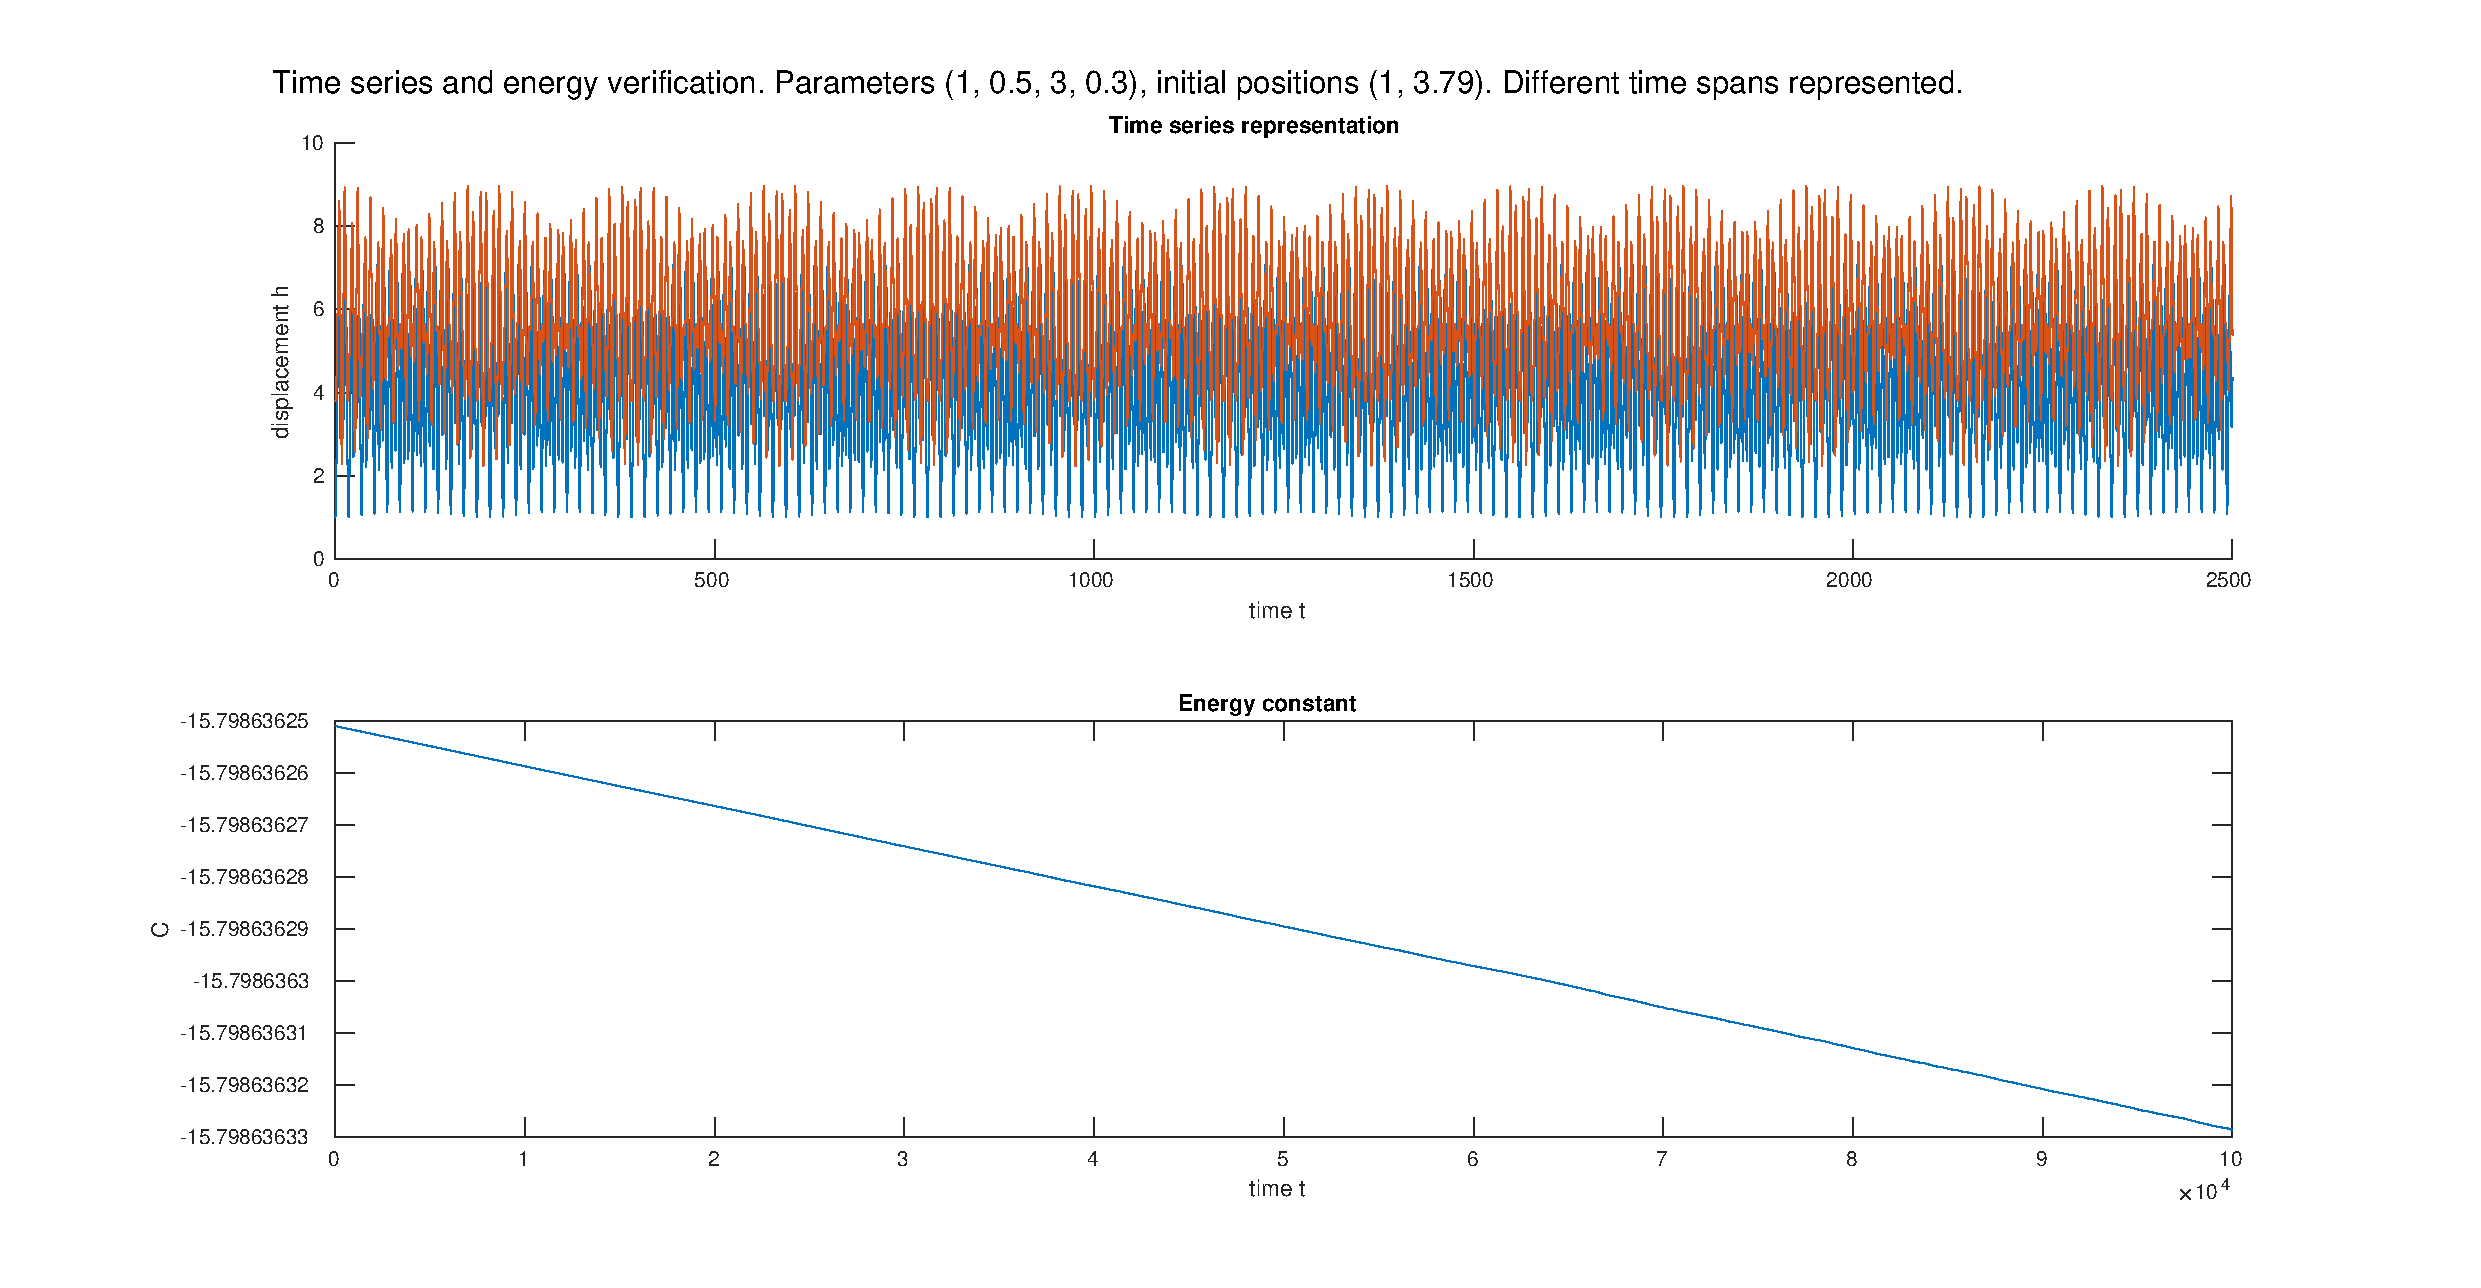
\includegraphics[width=\linewidth]{figures/twomass_energy_madplot_rev2.eps}
    \caption{
        Attempting to verify the result of nested orbits we have seen in Figure \ref{fig:twomass_nested_interesting_1}.
        The upper plot shows the same time series truncated at $t=3000$.
        The lower plot uses the energy constant defined in Equation \ref{eqn:twomass_energy_constant}.
        The energy constant accrues error from the initial conditions over the time span of the computation.
    }
    \label{fig:twomass_energy_madplot}
\end{figure}

\begin{figure}
    \centering
    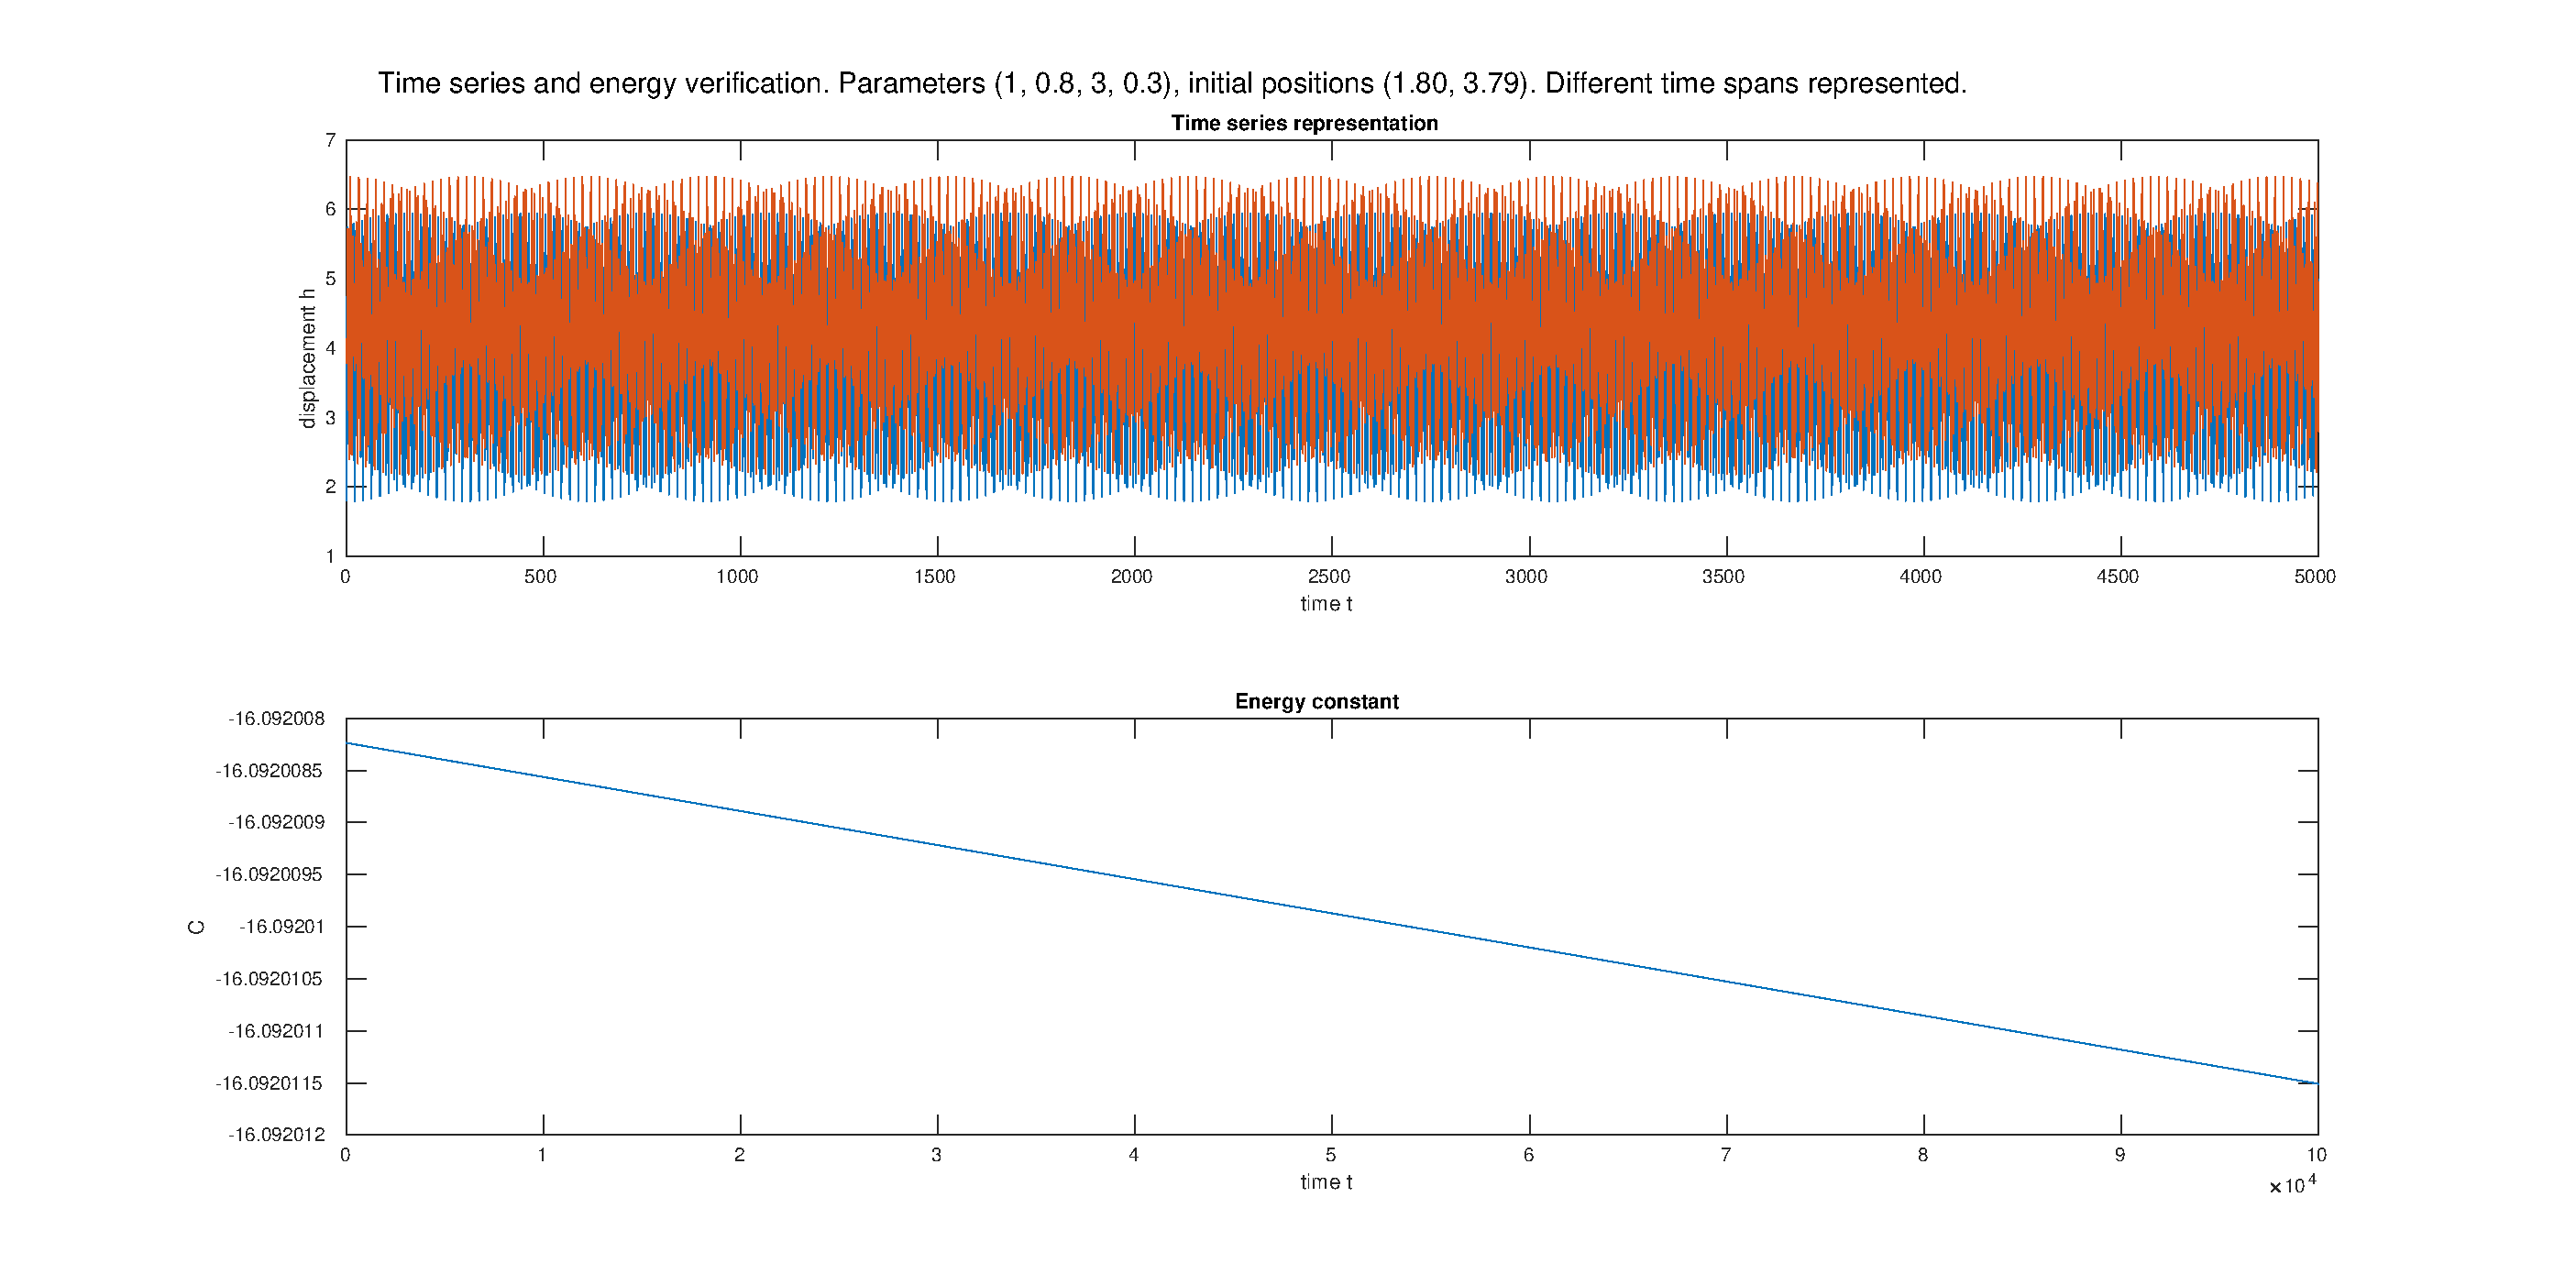
\includegraphics[width=\linewidth]{figures/twomass_timeseries_energy_comparison_2_rev1.eps}
    \caption{
        Second verification via energy constant.
        Parameters \((1, 0.8, 3, 0.3)\) with initial positions \((1.80, 3.79)\).
        The computation still diverges over time,
        although the rate at which the simulation loses energy is not as drastic as the earlier case.
    }
    \label{fig:twomass_energy_2}  %FIGURE CHANGED, FIX CAPTION
\end{figure}

\begin{figure}
    \centering
    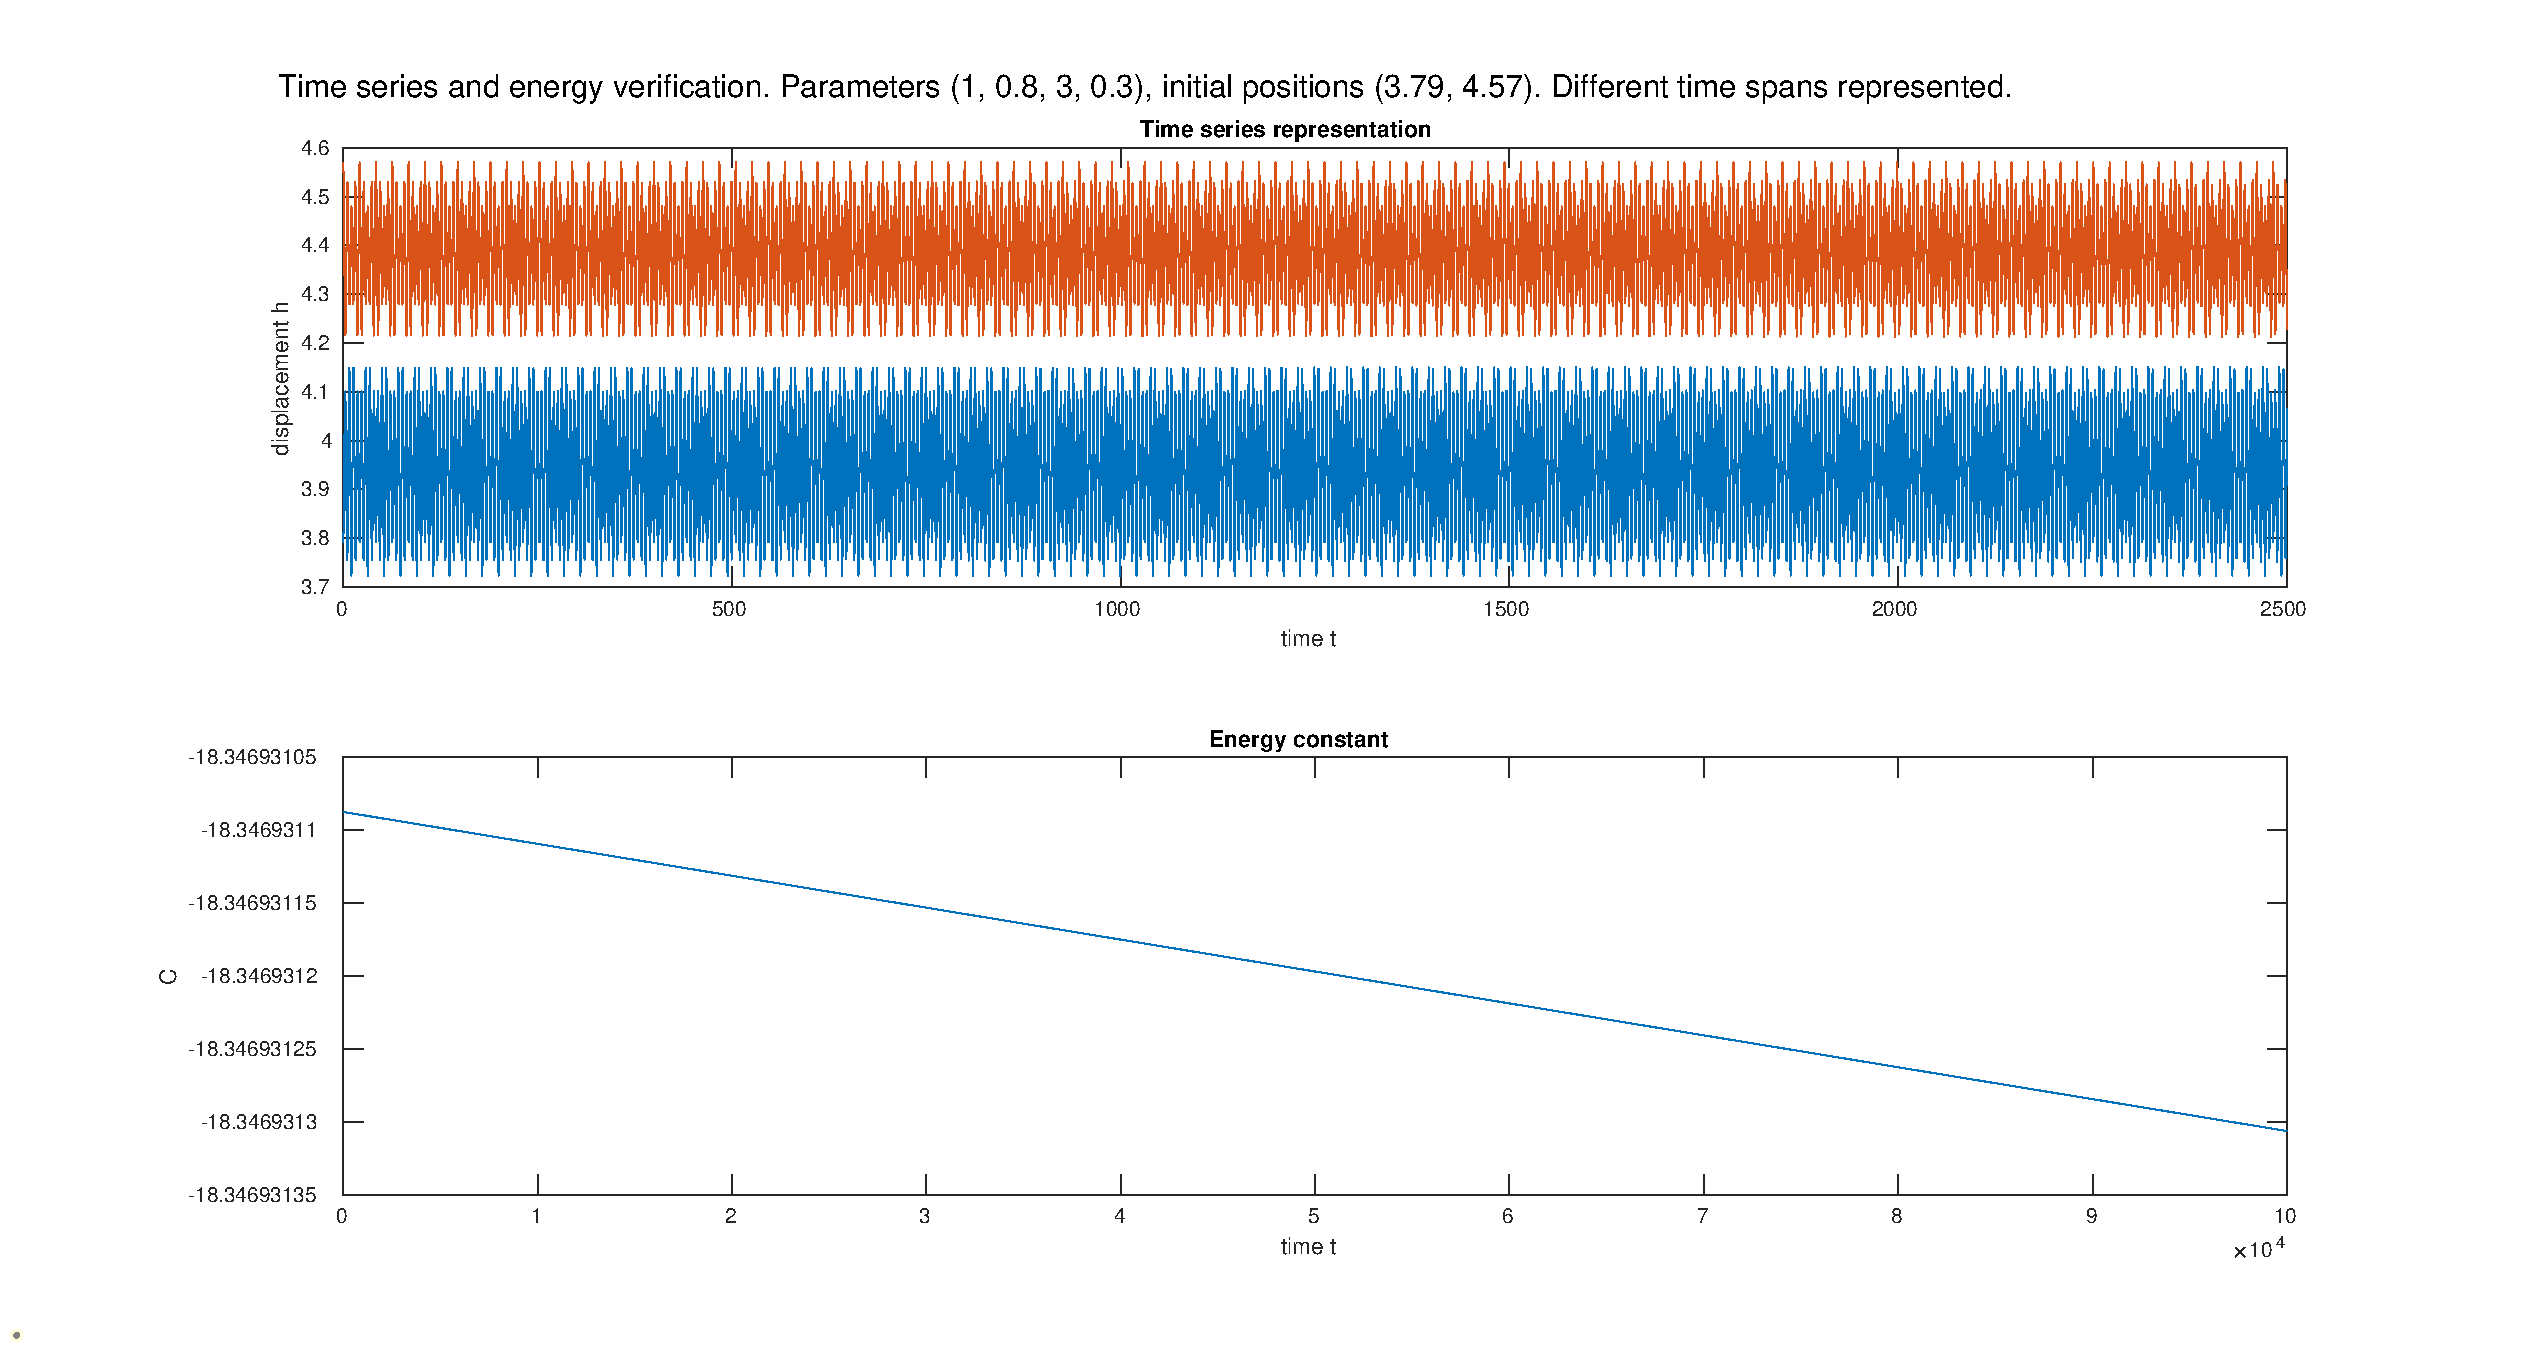
\includegraphics[width=\linewidth]{figures/twomass_timeseries_energy_verif_3_rev2.eps}
    \caption{
        Third verification via energy constant.
        Parameters \((1, 0.8, 3, 0.3)\) with initial positions \((3.79, 4.57)\).
        Regular, separate-bounded orbits.
        Under particular initial conditions, parameters, and time span,
        tbe system maintains a regular behaviour for which the energy constant is approximately maintained.
        See that the value of the energy constant doesn't change up to the first two decimal places.
        We have restricted the time span of the computation to force that the solution is more reliable than other results.
    }
    \label{fig:twomass_energy_3}
\end{figure}
We can also find a method of verification which relates to the energy of the system.
Recall the equations of motion which are given by Equation \ref{eqn:twomass_master_system}
We want to rearrange these equations and integrate, similar to what we did in the previous section, in order to find an expression that resembles the kinetic energy of the system.
First, we will write \(u = h_1,~v=h_2\) for convenience, and express the equations of motion in the form
\begin{align*}
    \frac{\mathrm{d}^2 u}{\mathrm{d}t^2} &= 1 - u + \beta\left(1-\frac{1}{u^2}\right) + \omega(v-u) \\
    \alpha\frac{\mathrm{d}^2 v}{\mathrm{d}t^2} &= \lambda(1 - v) + \beta\left(1-\frac{1}{v^2}\right) + \omega(u-v).
\end{align*}
Define functions $\hat{f}$ and $\hat{g}$ as follows
\begin{align*}
    \hat{f}(u) &= 1-u + \beta\left(1-\frac{1}{u^2}\right) \\
    \hat{g}(v) &= \lambda(1-v) + \beta\left( 1-\frac{1}{v^2} \right).
\end{align*}
Now define functions $F$ and $G$
\begin{align*}
    F(u) &= u - \frac{1}{2}u^2 + \beta\left(u - \frac{1}{u} \right) \\
    G(u) &= \lambda\left( v - \frac{1}{2}v^2 \right) + \beta\left( v - \frac{1}{v}\right).
\end{align*}
These functions satisfy \(\mathrm{d}F/\mathrm{d}u = \hat{f}(u)\) and \(\mathrm{d}G/\mathrm{d}v = \hat{g}(v)\).
We can write the system of differential equations in the form
\begin{align*}
    \frac{\mathrm{d}^2 u}{\mathrm{d}t^2} = \hat{f}(u) + \omega(v-u) \\
    \alpha\frac{\mathrm{d}^2 v}{\mathrm{d}t^2} = \hat{g}(v) + \omega(u-v).
\end{align*}
We will perform a rearranging of the expression on the second derivative of $u$,
but we will not go into detail on the derivation for the second expression,
since it is virtually identical.
First, we multiply the whole equation by the first derivative of $u$ with respect to $t$,
\begin{equation*}
    \frac{\mathrm{d}u}{\mathrm{d}t}\frac{\mathrm{d}^2 u}{\mathrm{d}t^2} = \frac{\mathrm{d}u}{\mathrm{d}t}\hat{f}(u) + \omega \frac{\mathrm{d}u}{\mathrm{d}t}(v-u).
\end{equation*}
This expression can be written mostly as derivatives, equivalently as
\begin{equation*}
    \frac{\mathrm{d}}{\mathrm{d}t}\left(
        \frac{1}{2}\left(\frac{\mathrm{d}u}{\mathrm{d}t}\right)^2
     \right) = \frac{\mathrm{d}}{\mathrm{d}t}F(u) - \omega\frac{\mathrm{d}}{\mathrm{d}t}\left(\frac{1}{2}u^2\right) + \omega v \frac{\mathrm{d}u}{\mathrm{d}t}.
\end{equation*}
Applying the same method to the second equation, we obtain
\begin{equation*}
    \frac{\mathrm{d}}{\mathrm{d}t}\left(
        \frac{1}{2}\alpha\left(\frac{\mathrm{d}v}{\mathrm{d}t}\right)^2
    \right) = \frac{\mathrm{d}}{\mathrm{d}t}G(v) - \omega\frac{\mathrm{d}}{\mathrm{d}t}\left( \frac{1}{2}v^2 \right) + \omega u \frac{\mathrm{d}v}{\mathrm{d}t}.
\end{equation*}
We would like to take the differential operator out of all the terms, but there are still mixed terms of $u$ and $v$ that make this difficult.
However, if we take the differential operator out of all the terms where we can, and ignore the mixed terms, we can add both expressions and obtain
\begin{equation*}
    \frac{\mathrm{d}}{\mathrm{d}t}\left(
        \frac{1}{2}\left(\frac{\mathrm{d}u}{\mathrm{d}t}\right)^2 + \frac{1}{2}\alpha\left(\frac{\mathrm{d}u}{\mathrm{d}t}\right)^2
    \right) = \frac{\mathrm{d}}{\mathrm{d}t}\left(
        F(u) + G(v) - \frac{\omega}{2}u^2 -\frac{\omega}{2}v^2
    \right) + \omega \left(
        u \frac{\mathrm{d}v}{\mathrm{d}t} + \frac{\mathrm{d}u}{\mathrm{d}t}v
    \right)
\end{equation*}
In adding both expressions, the mixed terms add together and form an integrable expression.
The expansion is given here:
\begin{equation*}
    \frac{\mathrm{d}}{\mathrm{d}t}(\omega uv) = \omega \left( u \frac{\mathrm{d}v}{\mathrm{d}t} + \frac{\mathrm{d}u}{\mathrm{d}t} v \right)
\end{equation*}
Hence the whole expression under the differential operator can be written as
\begin{equation*}
    \frac{\mathrm{d}}{\mathrm{d}t}\left(
        \frac{1}{2}\left(\frac{\mathrm{d}u}{\mathrm{d}t}\right)^2 + \frac{1}{2}\alpha\left(\frac{\mathrm{d}u}{\mathrm{d}t}\right)^2
    \right) = \frac{\mathrm{d}}{\mathrm{d}t}\left(
        F(u) + G(v) - \frac{\omega}{2}u^2 -\frac{\omega}{2}v^2 + \omega uv
    \right) 
\end{equation*}
and if we integrate the expression, and rearrange slightly, we obtain
\begin{equation}
    \frac{1}{2}\left(
        \left(\frac{\mathrm{d}u}{\mathrm{d}t}\right)^2 + \alpha \left(\frac{\mathrm{d}v}{\mathrm{d}t}\right)^2
    \right) = F(u) + G(v) - \frac{\omega}{2}(u-v)^2 + C.
    \label{eqn:twomass_energy_constant}
\end{equation}
This equation gives us an expression on the values \(u,~v,~\mathrm{d}u/\mathrm{d}t\) and \(\mathrm{d}v/\mathrm{d}t\),
which are the values we compute solutions of, and relates them to a constant $C$.
This is an energy constant, similar to what we derived in the earlier section on the single mass model.
Since the constant is unchanging in time, we can use it to verify that a computed solution is reliable,
by evaluating $C$ at multiple points in the time span of the computation.
Figure \ref{fig:twomass_energy_madplot} shows am attempted verification of a result using this constant.
Due to the nature of the integration method,
the energy constant accrues error over the time span of the computation.
The computation of the energy constant forms a curve which is fairly smooth,
however there is a large change in value,
which discredits the reliability of this result as an actual demonstration of the behaviour of the system.
Figures \ref{fig:twomass_energy_2} and \ref{fig:twomass_energy_3} show stronger results involving verification using the energy constant.
The variation in the result from Figure \ref{fig:twomass_energy_3} is bounded enough that we can claim it to be a stable result.

In our computation, even when the tolerances are extremely small,
the evaluations of the energy constant will always diverge slightly.
This occurs since the error of the numerical method is non-zero,
so an error accrues in the energy of the system.
Our criterion for a reliable solution is for the energy constant to be exact up to four decimal places.
When producing Figures \ref{fig:twomass_energy_madplot}, \ref{fig:twomass_energy_2} and \ref{fig:twomass_energy_3}, we have restricted the tolerances such that the solutions meet this criterion,
so that we can claim these results are reliable.

\subsection{The Poincar\'e map}

\begin{figure}
    \centering
    \includegraphics[width=0.9\linewidth]{figures/twomass_consistent_poincare.eps}
    \caption{
        The Poincar\'e map for the orbits represented earlier in Figure \ref{fig:twomass_nice_orbits_tspp}.
        Parameters \((1, 0.8, 3, 0.3)\) with initial positions \((3.79,4.57)\).
        The chosen hyperplane is the respective line where velocity is zero.
        The first plot is the Poincar\'e map for $h_1$ intersecting the line $\mathrm{d}h_1/\mathrm{d}t = 0$,
        where $v+$ indicates approaching the line with positive velocity.
        We can identify the intersection regions from the visualisation in the phase portrait in Figure \ref{fig:twomass_nice_orbits_tspp}.
        The transient is where we have plotted the intersection points against the order in which they were computed.
    }
    \label{fig:twomass_poincare_nice}
\end{figure}

Because the form of the problem is fourth order,
the problem can be analysed as the behaviour of an obejct in four dimensions.
The methods in which we have represented solutions graphically are simplifications,
where the four-dimensional behaviour is projected onto a two-dimensional image.

The Poincar\'e map is a useful technique we can use to analyse the behaviour of a system.
First, we construct the Poincar\'e section,
which is an $n-1$-dimensional subspace in the space that contains our solutions.
Another name for this type of subspace is a \textit{hyperplane}.
For a two dimensional problem, the Poincar\'e section is a line,
and for our current four dimensional problem it is a three-dimensional space.
The Poincar\'e map is the visualisation of the solution every time it intersects with the Poincar\'e section.
This can be used to assess quasiperiodicity or chaotic nature of dynamical systems.

In our case, we will consider the four dimensional problem as two separate two-dimensional problems,
which makes it easier to demonstrate the result.
We are essentially reducing the two mass model into two single mass models,
while acknowledging the coupling between them.
For our computations, the respective Poincar\'e sections for each mass are the lines in the phase portrait where their velocities are zero.

For the case of separate bounded continuous quasiperiodic orbits depicted in Figures \ref{fig:twomass_nice_orbits_tspp} and \ref{fig:twomass_energy_3},
we can construct the Poincar\'e map and analyse it in the context of the model.
Figure \ref{fig:twomass_poincare_nice} visualises the Poincar\'e map for this problem..
We see the intersection points begin to diverge as the computation continues,
shown in the visualisations that include the transient.
However, these diversions are small,
and the intersection points are mapped in clearly bounded regions.

The method used to compute the Poincar\'e map \cite{manohar_2011} constructs a new array of time points $T_n$ of intersections with the Poincar\'e section,
hence the figures do not plot to the same time scale as the original computations.

We have performed a similar computation of the Poincar\'e map in Figure \ref{fig:twomass_poincare_bad},
for a case we have explored earlier.
The points on the Poincar\'e map are much more irregular and break out of a pattern approximately halfway through the visualised computation.
This result is not reliable, justified again by the large scale of change in the energy constant we computed earlier in Figure \ref{fig:twomass_energy_madplot}.

The computations from the two mass model are, in general, very difficult to obtain reliable information from.
We cannot expect a numerical method to produce results which would match analytical behaviours.
However, it is sensible to deduce that there are families of behaviours that the model may exhibit,
which the numerical methods are incapable of reproducing.
For example, the computation shows that the initial quasiperiodic behaviour of Figure \ref{fig:twomass_nested_interesting_1},
which eventually settles to the stable equilibrium as shown in Figure \ref{fig:twomass_timeseries_settling},
can be shown to be invalid through computing the energy constant, shown in Figure \ref{fig:twomass_energy_madplot}.
Since the computation of the energy constant for this problem progressively decreases,
we could guess that the quasiperiodic motions will instead continue indefinitely, as shown in the early region of the time series.

\subsection{Unstable results}

\begin{figure}[h]
	\centering
	\includegraphics[width=\linewidth]{figures/twomass_individual_converging}
	\caption{
		Parameters given are \((1, 0.8, 3, 1)\). The masses oscillate near independently starting at different positions $(1.96, 0.83)$ at time $t=0$.
		The figures, left to right, progressively increase the time we run the computation.
		We can see in the left-most plot that the weak coupling leads to the masses oscillating at independent frequencies.
		As running time increases, the masses converge to their own equilibrium positions.
	}
	\label{fig:twomass_independent}
\end{figure}

\begin{figure}
	\centering
	\includegraphics[width=\linewidth]{figures/twomass_error_convergence.eps}
	\caption{
		Changes in solution as \(\mathtt{AbsTol}\) is decreased.
		Computations under parameters \((1, 0.8, 3, 1)\) with initial positions \((1.96, 0.83)\).
		The computed solution fundamentally changes under stepping down the tolerance.   
	}
	\label{fig:twomass_stepping_tolerance}
\end{figure}

\begin{figure}
	\centering
	\includegraphics[width=\linewidth]{figures/twomass_energy_comparison.eps}
	\caption{
		Solution from \texttt{ode45()} for the problem seen in Figures \ref{fig:twomass_nested_interesting_1} and \ref{fig:twomass_energy_madplot}.
		Without reducing the tolerance of the solver,
		the solution diverges.
	}
	\label{fig:twomass_energy_mistake}
\end{figure}

\begin{figure}
	\centering
	\includegraphics[width=0.9\linewidth]{figures/twomass_poincare_map.eps}
	\caption{
		Another example of the Poincar\'e map, for the computation shown earlier in Figures \ref{fig:twomass_timeseries_settling}, \ref{fig:twomass_nested_interesting_1} and \ref{fig:twomass_energy_madplot}.
		We have shown that this result is not reliable, since we can compute that the energy constant diverges.
		As we can see, the orbits break out of a pattern and the points on the Poincar\'e map begin to converge.
	}
	\label{fig:twomass_poincare_bad}
\end{figure}

The numerical solver struggles with the unstable equilibrium solutions,
since near these points, the ODE is extremely sensitive to minute differences in the numerical values.
Due to finite precision floating point arithmetic,
it is extremely difficult to produce consistent results near the unstable equilibria numerically.
In combination with the stiffness coupling, there are often heavily unbalanced forces on each mass,
for example if an unstable equilibrium lies between the two masses.
Figures \ref{fig:twomass_energy_mistake} and \ref{fig:twomass_poincare_bad} show analysis of computations where the behaviour has diverged from a consistent result.
The time series slowly breaks out of quasiperiodic orbits and begins to converge towards a stable equilibrium,
while the reliable solution in Figure \ref{fig:twomass_energy_madplot} shows continuous quasiperiodic behaviour.

Figure \ref{fig:twomass_stepping_tolerance} shows a change in results when reducing the $\mathtt{AbsTol}$ parameter for the MATLAB \texttt{ode45()} function.
The figures show that decreasing the error tolerance can fundamentally change the numerical solution,
especially where closure is not observed for tolerance of order $10^{-5}$,
but is observed for $10^{-10}$.
Recall that $\mathtt{AbsTol}$ is a lower bound on the magnitude of the solution that MATLAB will compute.
Clearly, the closure of the model, being the case of a mass approaching zero,
is affected by how MATLAB handles solutions that approach zero.

\section{Voiced sounds}

\begin{figure}
	\begin{subfigure}[b]{0.5\textwidth}
		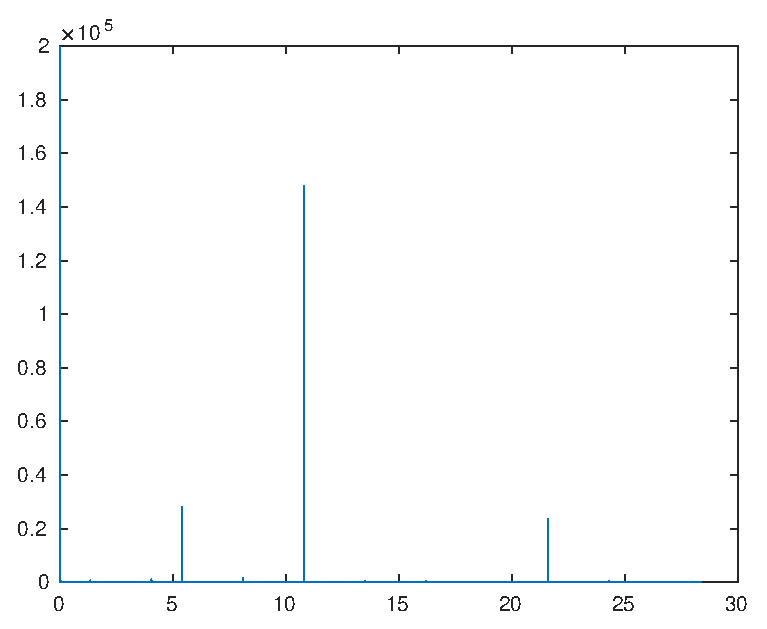
\includegraphics[width=\textwidth]{voiced_sounds/case_1/most_stable_resulta.eps}
	\end{subfigure}
	\begin{subfigure}[b]{0.5\textwidth}
		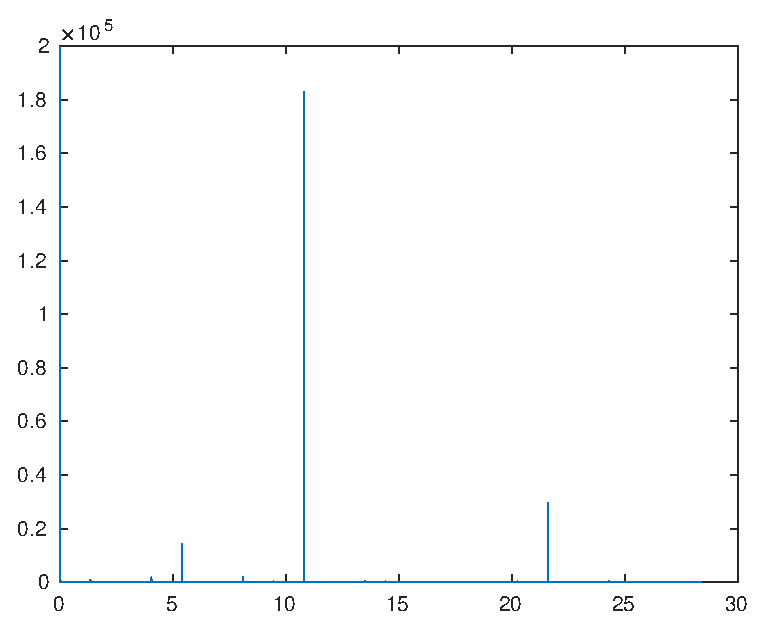
\includegraphics[width=\textwidth]{voiced_sounds/case_1/most_stable_resultb.eps}
	\end{subfigure}
	\caption{
		Fourier transforms of time series data from same conditions as Figure \ref{fig:twomass_energy_3}, with extended time span.
		Left is $h_1$, right is $h_2$ with parameters \((1, 0.8, 3, 0.3)\) and initial positions $(3.79,4.57)$.
		We can identify similar spectra of different magnitude,
		particularly three distinct spikes with the middle value being the most powerful.
	}
	\label{fig:twomass_fourier_first}
\end{figure} % same as energy madplot

\begin{figure}
    \begin{subfigure}[b]{0.5\textwidth}
        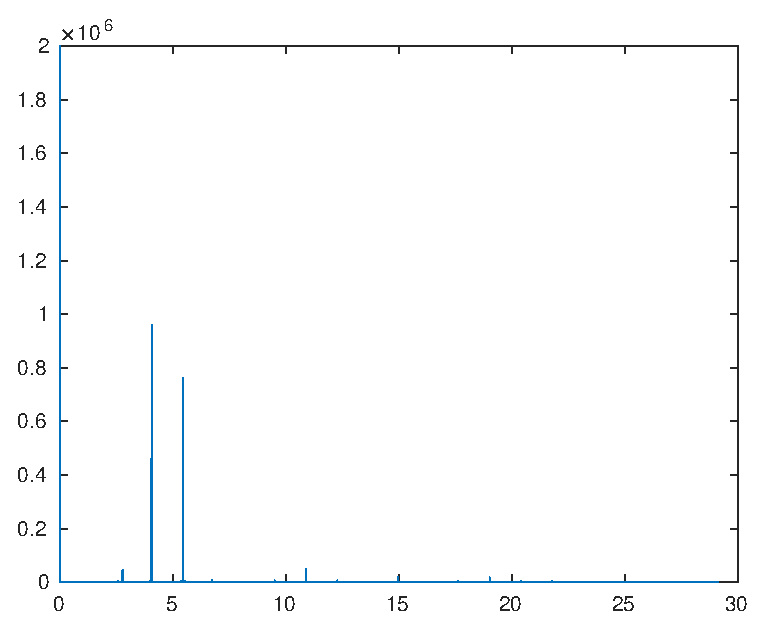
\includegraphics[width=\textwidth]{voiced_sounds/case_2/other_stable_resulta.eps}
    \end{subfigure}
    \begin{subfigure}[b]{0.5\textwidth}
        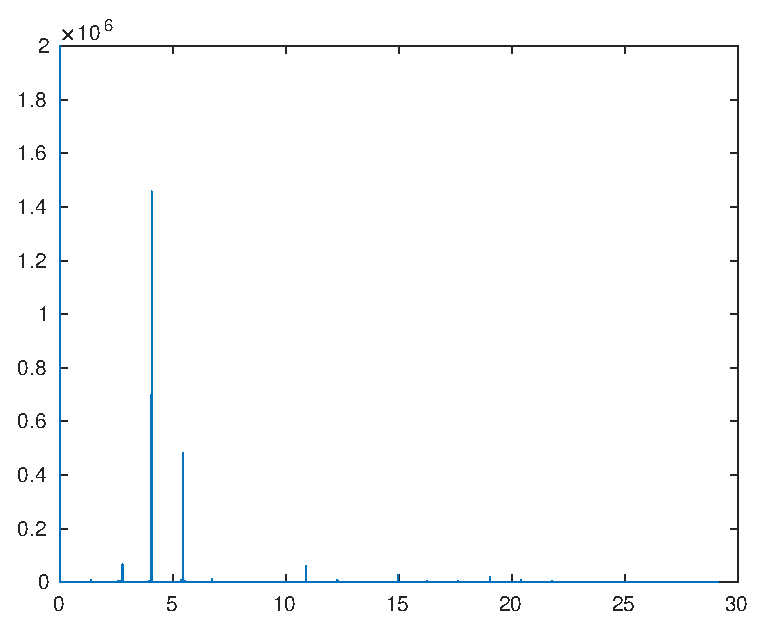
\includegraphics[width=\textwidth]{voiced_sounds/case_2/other_stable_resultb.eps}
    \end{subfigure} %% same as energy 2
    \caption{
        Fourier transforms of time series data instead from Figure \ref{fig:twomass_energy_2}, again with extended time span.
        Presentation is identical to the prior figure.
        Parameters \((1, 0.8, 3, 0.3)\) and initial positions $(1.80,3.79)$.
        Quasiperiodic orbits that intersect.
        The dominant frequencies of oscillation are close together,
        but the weighting of these frequencies is extremely different in both.
    }
    \label{fig:twomass_fourier_second}
\end{figure}

\begin{figure}
	\begin{subfigure}[b]{0.5\textwidth}
		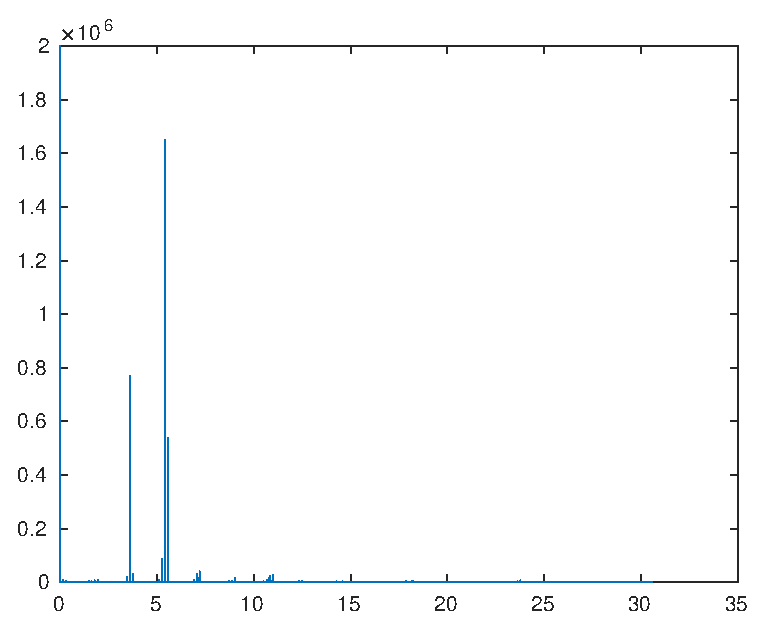
\includegraphics[width=\textwidth]{voiced_sounds/case_3/interesting_quasi_a.eps}
	\end{subfigure}
	\begin{subfigure}[b]{0.5\textwidth}
		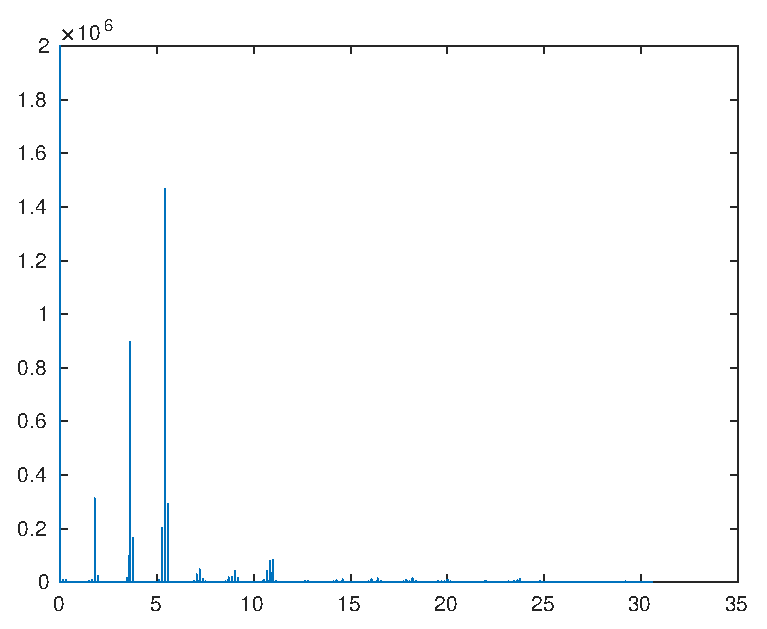
\includegraphics[width=\textwidth]{voiced_sounds/case_3/interesting_quasi_b.eps}
	\end{subfigure}
	\caption{
		Fourier transforms of extended time series data from Figure \ref{fig:twomass_energy_madplot}.
		Vertical axis is the power of frequencies on the horizontal.
		Frequency ranges from $0$ to $n/T$ where $n$ is the number of time points and $T$ is the end time of the computation.
		We computed the solution initialised with parameters \((1, 0.5, 3, 0.3)\) and initial positions \((1,3.79)\).
		The continuous quasiperiodic orbits provide a far richer visualisation than the prior two examples,
		where we can identify clusters of frequencies rather than distinct single spikes of intensity.
	}
	\label{fig:twomass_fourier_madplot}
\end{figure}

We can generate playable sound files in \texttt{.wav} format of the time series computations,
and we can play these back to hear our results.
Sound files are generated by interpolating the time series into an array with uniform timestep,
normalising the range to $[-1,1]$
and then using the \texttt{audiowrite()} function in MATLAB to write the array to a \texttt{.wav} file.
We generate two separate audio files for the motion of each mass.
Playable sound files are available \hyperlink{https://gitlab.com/willwoolfenden/undergraduate-project-2223-phonation}{here}\footnote{https://gitlab.com/willwoolfenden/undergraduate-project-2223-phonation},
with three results each containing a time series graph we have shown,
and two playable sound files for each mass.

A Fourier transform can be applied to the original time series data to provide information on the frequencies of the oscillations.
Figures \ref{fig:twomass_fourier_first},
\ref{fig:twomass_fourier_second} and \ref{fig:twomass_fourier_madplot} apply the transform to data we are familiar with,
having extended the time scale.
Frequency space is computed as the $n$ points in the time array divided by the total time span.
Since the time series data is produced by a non-uniform timestep,
we use the \texttt{nufft()} function in MATLAB,
which is a non-uniform fast Fourier transform algorithm that requires the time series array and the time array as arguments.
We apply the Fourier transform to the positions of $h_1$ and $h_2$ in the time series.

On long time scales, solutions may diverge from a consistent behaviour if we do not control the tolerance of the numerical solver.
The results provided are computed with the settings $\mathtt{AbsTol}=10^{-40}$ and $\texttt{RelTol}=10^{-12}$.
The Fourier transform graphs are all results which have been studied earlier,
and are all available in the repository.

In all the Fourier transform visualisations we have available,
we can identify similar spectra between the masses.
Figures \ref{fig:twomass_fourier_first} and \ref{fig:twomass_fourier_second} visualise frequency spectra with discrete spikes.
The first plot shows the two masses oscillate with identical frequencies,
and the strength of these frequencies are very close in both.
In the second, smaller spikes in frequency information do appear more often,
which can describe more complex behaviour of the masses.
In Figure \ref{fig:twomass_fourier_madplot},
the spectral information is much richer,
where frequencies cluster together instead of being distinct spikes.
The form of this Fourier transform representation describes much more complex motion of the masses than the other cases we have shown.

\bibliographystyle{unsrt}
\bibliography{sources.bib}

\end{document}

